% ============================================================
% Personalized Behavioral Drift Detection for Fair and
% Explainable Online Exam Integrity
% ACM sigconf format (LAK 2027)
% ============================================================
% Use [sigconf,draft] to compile FAST (skips image rendering).
% Remove `draft` only for the final build.
\documentclass[sigconf]{acmart}

% Suppress PDF page group warnings (speeds things up a bit)
\pdfsuppresswarningpagegroup=1

% ---- Packages ----
% acmart already loads amsmath, amsfonts, amssymb via newtxmath.
% Loading amssymb again causes a \Bbbk clash.
\let\Bbbk\relax          % avoid clash between newtxmath and amssymb
\usepackage{amsmath,amssymb}
\usepackage{graphicx}
\usepackage{booktabs}
\usepackage{multirow}
\usepackage{array}
\usepackage{url}

\graphicspath{{figures/}}

% ---- ACM metadata ----
\copyrightyear{2027}
\acmYear{2027}
\setcopyright{acmlicensed}
\acmConference[LAK '27]{Proceedings of the 17th International Conference on Learning Analytics and Knowledge}{March 2027}{venue to be announced}
\acmBooktitle{Proceedings of the 17th International Conference on Learning Analytics and Knowledge (LAK '27), March 2027, venue to be announced}
\acmDOI{10.1145/nnnnnnn.nnnnnnn}
\acmISBN{978-x-xxxx-xxxx-x/27/03}

\begin{document}

% ---- Title ----
\title{Personalized Behavioral Drift Detection for Fair and Explainable Online Exam Integrity}

% ---- Authors ----
\author{Srivathsa H}
\affiliation{%
  \institution{BITS Pilani Dubai Campus}
  \city{Dubai}
  \country{UAE}
}
\email{f20230198@dubai.bits-pilani.ac.in}

\author{Mili Mohan}
\affiliation{%
  \institution{BITS Pilani Dubai Campus}
  \city{Dubai}
  \country{UAE}
}
\email{f20230293@dubai.bits-pilani.ac.in}

\author{Irene M}
\affiliation{%
  \institution{BITS Pilani Dubai Campus}
  \city{Dubai}
  \country{UAE}
}
\email{f20230026@dubai.bits-pilani.ac.in}

\author{Kalyani B S}
\affiliation{%
  \institution{BITS Pilani Dubai Campus}
  \city{Dubai}
  \country{UAE}
}
\email{f20230236@dubai.bits-pilani.ac.in}

% ============================================================
% ABSTRACT
% ============================================================
\begin{abstract}
Online examinations have now become the new normal for higher
education institutions across the globe. However, the tools we use to ensure the integrity of these online examinations are still in the development stages. Most of the tools rely on intrusive webcam surveillance or the use of strict rule-based triggers that treat all students the same. These tools are based on the notion that all students have the same examination patterns, which is not the case. These tools are also based on the fact that some demographics are more prone to being flagged than others. In this paper, we propose a new framework for detecting cheating in online examinations. Instead of focusing on the student’s appearance during the examination, we have developed a new method of modeling the student’s typical
behavior during the examination based on the student’s clickstream data.  Our detector is a Transformer-based supervised classifier that works at the per-action level and asks ``does this session show the same behaviour pattern as the rest?'' Flagged sessions go through a threshold calibration step, taking into consideration four demographic dimensions: gender, age, IMD, and disabilities. Explanations produced using SHAP value provide information about individual questions that triggered flags. We evaluate on $\sim$15{,}000 students sampled from the EdNet-KT2 clickstream dataset, augmented with OULAD demographic profiles and GAN-enhanced synthetic anomalies grounded in the literature on cheating behaviour. The proposed Transformer achieves ROC-AUC $0.959$ ($95\%$ CI $[0.950, 0.968]$), recall $0.894$, and precision@10 $= 1.00$ on a held-out test split composed entirely of synthetic anomalies grounded in the cheating-behaviour literature, with detection performance comparable to a strong supervised BiLSTM baseline and substantially better than Isolation Forest, One-Class SVM, a feed-forward autoencoder, a rule-based detector, and an LSTM autoencoder. These figures should be understood as an upper bound under regulated conditions rather than as approximates of real-world detection performance. After per-group threshold calibration applied to synthetically sampled demographic groups from OULAD marginal distributions, all four demographic axes achieve DPR $= 1.00$ and EOD $= 0.00$ on the test split, validating calibration mechanism rather than demonstrating fairness on a natural demographic variation. A Streamlit prototype dashboard presents ranked anomaly scores, exam timelines, and SHAP-based explanations for instructor review.
\end{abstract}

% ---- CCS Concepts ----
\begin{CCSXML}
<ccs2012>
   <concept>
       <concept_id>10010147.10010257.10010293.10010294</concept_id>
       <concept_desc>Computing methodologies~Neural networks</concept_desc>
       <concept_significance>500</concept_significance>
   </concept>
   <concept>
       <concept_id>10010147.10010257.10010293.10010319</concept_id>
       <concept_desc>Computing methodologies~Learning latent representations</concept_desc>
       <concept_significance>500</concept_significance>
   </concept>
   <concept>
       <concept_id>10003120.10003145.10003147.10010919</concept_id>
       <concept_desc>Human-centered computing~Empirical studies in collaborative and social computing</concept_desc>
       <concept_significance>300</concept_significance>
   </concept>
   <concept>
       <concept_id>10010405.10010462</concept_id>
       <concept_desc>Applied computing~Education</concept_desc>
       <concept_significance>500</concept_significance>
   </concept>
</ccs2012>
\end{CCSXML}

\ccsdesc[500]{Computing methodologies~Neural networks}
\ccsdesc[500]{Computing methodologies~Learning latent representations}
\ccsdesc[300]{Human-centered computing~Empirical studies in collaborative and social computing}
\ccsdesc[500]{Computing methodologies~Supervised learning}
\ccsdesc[500]{Applied computing~E-learning}

% ---- Keywords ----
\keywords{behavioral drift detection, online exam integrity, Transformer, GAN, anomaly detection, clickstream analysis, fairness in AI, explainable AI, learning analytics}


\maketitle

% ============================================================
% 1. INTRODUCTION
% ============================================================
\section{Introduction}

Remote examinations are, by now, a standard feature of higher education. The shift accelerated during the COVID-19 pandemic~\cite{coghlan2021good}, but it was already underway before 2020 and it shows no signs of reversing. The issue is simple: the traditional approach to invigilation doesn't function when the student is sitting the exam at home rather than in a lecture theater. The universities have responded to
this by using computerized invigilation systems, but the options
available are, for the most part, disappointing.

The most widely used commercial proctoring systems like ProctorU, ExamSoft, Respondus LockDown Browser, rely heavily on webcam feeds, screen recording, and audio capture~\cite{nigam2021systematic}.These tools come with well-documented concerns. They create a confrontational relationship between students and computers and there is so much surveillance in these test environments. Serious concerns exist about student privacy and other student-related issues, such as the fact that there is a high rate of false positives for students of color, students with disabilities, and students in non-standard testing conditions~\cite{swauger2020software}. And they are reactive, watching students rather than actually understanding what they are doing.

On the research side, clickstream analytics has been used extensively to study student engagement, predict performance, and identify at-risk learners in learning management systems~\cite{gardner2019evaluating, aljohani2019predicting, brinton2015mooc}. This body of work is valuable, but it mostly focussed on patterns at the course level over period of weeks or months, like how often a student logs in or how many posts they read in the forum,etc. Exam integrity monitoring is a different problem. It requires temporally fine-grained modeling at the question level within a single exam session.


A few studies have applied anomaly detection methods to cheating in MOOCs~\cite{ruiperez2017detection, alexandron2019fraud} and collusion in programming assignments~\cite{li2015detecting}. These methods usually use a statistical baseline for the general population to find the student who stands out from the rest. The problem is that students \textit{are} different from one another. Some people naturally think things through more carefully, go back to questions more often, or answer them out of order. Any detector that uses the same average for everyone will always misclassify honest students who are just a little different from the average.

\smallskip
\noindent\textit{Why personalized drift matters --- a concrete example.} Consider a student whose normal pattern is to answer every question in $10$--$15$ seconds with very low response-time variance, simply because they prefer to commit quickly and move on. A population-based detector, calibrated against a global mean response time of $30$ seconds, will repeatedly flag this student as suspicious in every exam they take. Our framework instead asks whether \emph{this} session looks different from \emph{this} student's prior sessions: the same fast-and-uniform pattern that looks anomalous against the population looks perfectly normal against the student's own history, and is no longer flagged. Conversely, if the same student suddenly produces a session with long pauses followed by bursts of compressed answers, the personalized baseline notices the deviation immediately, even though that pattern is unremarkable in the population average.

From a learning analytics perspective, this work operationalizes behavioral consistency as a proxy for authentic engagement, based on self-regulated learning frameworks~\cite{zimmerman2002becoming} and the long-standing argument in the LAK community that integrity tools should support student learning instead of simply punishing them~\cite{baker2010data,khosravi2022explainable}. Treating each session as a behavioural trace to be understood, rather than a surface to be policed, aligns with that pedagogical stance.

This paper proposes a framework built around a different idea: \textbf{personalized behavioral drift detection}. Instead of asking, ``Does this student look different from other students?'' we ask, ``Does this session look like a normal behavioural sequence?'' and for students with enough history, ``Does this session look different from this student themselves?''. The proposed detector is a supervised Transformer classifier trained end-to-end on behavioural sequences with synthetic anomaly labels. We also look at two problems that are often ignored in the literature on anomaly detection at the same time:

\begin{enumerate}
    \item \textbf{Fairness.} It is easy for anomaly detection systems to encode demographic biases. A naive system will be unfair to students in certain groups if they tend to have higher values in the drift metrics because of differences in testing environments, access to devices, and cultural patterns. We make fairness a part of the detection pipeline by calibrating the threshold for each group.
    \item \textbf{Explainability.} An opaque score doesn't help a teacher decide whether or not to look into a flag. We give SHAP-based explanations for each flagged session at the feature level, which shows \textit{which} behavioural features (e.g., answer-change frequency, time per question) caused the flag.
\end{enumerate}

Concretely, our contributions are:
\begin{itemize}
    \item A Transformer-based supervised detector that operates on action-level clickstream sequences with an inference-time per-student blending step (Eq.~$4$), giving genuinely \emph{personalised} drift scores while still benefiting from supervised training; on the synthetic-anomaly evaluation it reaches ROC-AUC $0.959$ ($95\%$ CI $[0.950, 0.968]$) and recall $0.894$, comparable to a strong BiLSTM baseline and substantially better than the unsupervised baselines.
    \item  A behavioural feature extractor that creates sequential model (per-question level) and classical model (session level) features.
    \item A GAN-augmented synthetic-anomaly pipeline seeded by literature-grounded rule-based anomalies, used to create a realistic training signal in the absence of labelled cheating data.
    \item A post-hoc fairness-aware threshold calibration mechanism that achieves DPR $\geq 0.80$ and EOD $\leq 0.10$ across gender, age band, IMD band, and disability status.
    \item A SHAP-based explainability component that produces question-level and feature-level attributions for each flag, and a Streamlit prototype dashboard that combines anomaly scores, the exam timeline, and these explanations.
    
\end{itemize}
\noindent\textbf{Source code.} The full implementation, training scripts, synthetic anomaly pipeline, and dashboard prototype are released at \url{https://github.com/f20230198-art/PERSONALIZED-BEHAVIORAL-DRIFT-DETECTION-FOR-FAIR-AND-EXPLAINABLE-ONLINE-EXAM-INTEGRITY}.


% ============================================================
% 2. RELATED WORK
% ============================================================
\section{Related Work}
\label{sec:related}

We organise prior work into five threads that, together, motivate the design of our framework.

\subsection{Automated Online Proctoring}
Proctoring applications for commercial purposes have become increasingly popular as more individuals opt for online classes. The use of features such as web camera face tracking, eye movement analysis, and screen locking may assist in detecting whether any malpractices have occurred during your exam through audio surveillance.~\cite{nigam2021systematic}. Though effective at deterrence, such platforms have faced intense scrutiny. Swauger~\cite{swauger2020software} documents how algorithmic proctoring disproportionately affects students with darker skin tones, physical disabilities, and atypical testing environments. Coghlan et al.~\cite{coghlan2021good} these technologies represent a problematic approach to surveillance referred to as "Big Brother". We propose to avoid such methods and use only anonymized clickstream data instead.

\subsection{Clickstream and Behavioural Analytics in Education}
Clickstream analysis is one of the oldest techniques in educational data mining. Baker and Yacef~\cite{baker2010data} use of interaction logs for evaluating off-task behavior in intelligent tutoring systems was explored early on. More recently, EdNet~\cite{choi2020ednet},The public repository dataset is composed of the millions of clicks in educational problem solving with information on the location, timestamp and changes made to the problem attempted. Brinton and Chiang~\cite{brinton2015mooc} showed that fine-grained clickstream features could predict engagement and dropout in MOOCs; Aljohani et al.~\cite{aljohani2019predicting} applied similar ideas to virtual learning environments using OULAD~\cite{open_university_learning_analytics_dataset_349}. Hussain et al.~\cite{hussain2018student} Clickstream data was enriched using engagement measures through the interaction log, concentrating more on engagement within the course than any behavior anomaly during the exam.

\subsection{Anomaly Detection for Academic Integrity}
Several groups have worked on anomaly detection for academic dishonesty. Ruiperez-Valiente et al.~\cite{ruiperez2017detection} statistical analysis was performed on MOOC test evaluations, specifically on time taken to complete the test and similarity in responses among students; Alexandron et al.~\cite{alexandron2019fraud} extended this with a more systematic analysis of harvesting and copying; Li and Zhai~\cite{li2015detecting} used clustering to flag collusion in programming assignments. On the methods side, Isolation Forest~\cite{liu2008isolation} and One-Class SVM~\cite{scholkopf2001estimating} remain widely used baselines. Malhotra et al.~\cite{malhotra2016lstm} the study reveals that LSTM-based architectures show good results in detecting anomalies in multivariate time series data, which are structurally similar to exam clickstreams and Chalapathy and Chawla~\cite{chalapathy2019deep} following this, a more extensive review of deep anomaly detection techniques is conducted. Recently, Transformers have become the standard sequence models used in all fields where they are applied.~\cite{vaswani2017attention}, we use these components as our primary detector. The key differences of this paper compared to previous research are as follows: (i) the use of Transformer-based supervised sequence detector with the ability to recognize literature-based anomalies synthesized within an exam integrity framework, and (ii) the introduction of drift normalization, which, when sufficient data is available, compares students against their personal mean instead of the mean for all people.

\subsection{Fairness in Educational AI}
Fairness is a first-order concern in automated educational tooling. Baker and Hawn~\cite{baker2022algorithmic} offers an extensive review of algorithmic discrimination within the context of education, with special consideration of predictive modeling, recommendation algorithms, and automated testing; Kizilcec and Lee~\cite{kizilcec2022algorithmic} it highlights how the use of algorithms may further exacerbate existing forms of injustice, especially those related to race and socioeconomic status; Gardner et al.~\cite{gardner2019evaluating} Despite having highly successful predictive models, there exist significant differences in their performance between various demographics. In anomaly detection specifically, Zhang and Davidson~\cite{zhang2021fair} developed fairness-aware methods for unsupervised settings; Mehrabi et al.~\cite{mehrabi2021survey} survey fairness definitions and mitigation strategies across ML. Holstein et al.~\cite{holstein2019improving} there is an agreement among practitioners that considerations related to fairness should not be seen as secondary, but rather as one of the primary goals of design.

\subsection{Explainable AI in Education}
The use of explainable AI systems in education is necessary both from a practical and moral standpoint because teachers need to know how things work \textit{why} a flag was raised before acting on it. Khosravi et al.~\cite{khosravi2022explainable} argue that explainable AI is essential for trust and meaningful human oversight. SHAP~\cite{lundberg2017unified},based on Shapley values in cooperative game theory, this methodology has become one of the most popular tools for explaining features.; Swamy et al.~\cite{swamy2022evaluating} various interpretability techniques were assessed for their effectiveness in predicting MOOC student performance, with SHAP emerging as the most reliable one.
Doshi-Velez and Kim~\cite{doshivelez2017towards} a general methodology was devised to assess the criteria for interpretability, thus providing motivation for presenting both question-level and feature-level SHAP interpretations. Moreover, we would like to emphasize that to the best of our knowledge, ours is the first comprehensive platform that uses a supervised Transformer model with post-hoc fairness evaluation and SHAP explanations in online examinations.

% ============================================================
% 3. PROPOSED FRAMEWORK
% ============================================================
\section{Proposed Framework}
\label{sec:proposed}

The architecture of the proposed system is depicted in Figure~\ref{fig:system_overview}. The first step is to obtain the EdNet clickstream dataset to extract behavioral features from it. Then, the features are provided to a pre-trained Transformer-based classifier along with other baseline models to evaluate them against each other. Once the classifiers predict scores, they are filtered using a threshold to classify them into decisions. These decisions are calibrated for better fairness results, and then SHAP explanations are obtained.

\begin{figure}[htbp]
\centering
\fbox{\parbox{0.92\columnwidth}{\centering\vspace{1.0em}Raw Clickstream $\rightarrow$ Feature Extraction $\rightarrow$\\[0.3em]
\{ Transformer Classifier \,\textbf{(Ours)}\ \,$|$\, Baselines \}\\[0.3em]
$\rightarrow$ Drift Score $\rightarrow$ Fairness Calibration $\rightarrow$ SHAP Explanations $\rightarrow$ Dashboard\vspace{1.0em}}}
\caption{Overview of the proposed behavioural drift-detection framework. Clickstream data flows through feature extraction, detection (Transformer classifier as the main proposed model, alongside classical and sequence baselines), fairness-aware threshold calibration, and SHAP-based explainability.}
\label{fig:system_overview}
\end{figure}

\subsection{Behavioural Feature Extraction}
For each exam session we extract two parallel views of the same clickstream:

\paragraph{Session-level features (10 features, flat vector).} These factors form the basis of comparison, which include rules-based methods, Isolation Forest, One-Class SVM, and traditional autoencoders. The session is presented as a vector obtained by summarizing the properties related to time, uncertainty, and navigation. In particular, the list of features includes statistical properties of the distribution of response time (average, variance, interquartile range, and entropy), the percentage of questions whose answers have been altered, keystroke rhythm, pause time, the percentage of re-visited questions, and speed peaks.

\paragraph{Action-level sequence features (10 features $\times$ up to 100 actions).} Utilized in sequence models (Transformer, LSTM-AE, and BiLSTM). The attributes of each action include the interaction gap in both its raw and log-normalized forms, the $z$-score of the gap for the session, the indicator of answer change, an indicator to show whether the current question is the same as the previous question, the normalized question number, the normalized action number in the session, the number of previous actions taken for the current question, the fraction of time passed in the session, and a long pause indicator (gap $>$ 30 s). All these features are normalized by $z$-score based on statistics calculated on the training set \emph{clean} data only.

The dual-view design was created intentionally, where sequence models rely on temporal ordering to assess data, while session-level vectors facilitate the baseline comparisons of traditional systems

\subsection{Main Proposed Detector: Transformer Classifier}
The primary detector used is a supervised Transformer encoder with a classification head. In case of an input sequence $\mathbf{X} \in \mathbb{R}^{T \times F}$ ($T \le 100$ actions, $F = 10$ features) per action, this input is mapped to a $d_{\text{model}}$-dimensional space. Next, a position embedding learned by the model is used and passed through Transformer encoder layers with attention masks in place. The next step involves performing a mean-pooling operation using masking over all valid positions, thus creating a session embedding. This embedding is finally passed through a two-layer MLP head to produce one anomaly logit score:
\begin{align}
\mathbf{H} &= \text{TransformerEncoder}\bigl(\mathbf{X}\mathbf{W}_{\text{in}} + \mathbf{P},\, \text{pad\_mask}\bigr),\\
\mathbf{z} &= \text{MaskedMean}(\mathbf{H}),\\
\hat{y} &= \sigma\bigl(\text{MLP}(\mathbf{z})\bigr) \in (0,1).
\end{align}
Our model uses a configuration of $d_{\text{model}} = 128$, $4$ attention heads, $3$ encoder layers, and dropout $0.2$. We train the network with Adam optimization and binary cross-entropy loss with respect to our anomaly label, which considers a positive class weight proportional to the number of negative to positive samples, while also using gradient clipping ($\lVert g \rVert \le 1$). Early stopping with a patience of 10 epochs was used, based on the validation loss. Our self-attention framework is believed to have a better inductive bias compared to a pure recurrent approach due to the possible dependence between actions in terms of cheating behavior at the level of actions, for example, where there may be a pattern of increasing reply rates in the later part of a session based on the relative position of questions.

\paragraph{Personalised inference-time scoring.} The Transformer above is trained as a population-level supervised classifier. To honour the ``personalised drift'' framing of the paper, we apply a per-student blending step at \emph{inference time} on the Transformer's raw logit $\hat{y}_s$ for session $s$ of student $u$. Let $\bar{y}_u$ and $\sigma_u$ denote the median and (robust) MAD-scaled spread of the model's logits over student $u$'s clean training sessions, and let $\bar{y}_{\text{pop}}$, $\sigma_{\text{pop}}$ be the corresponding population statistics computed on all clean training sessions. The blended drift score is
\begin{equation}
D(s) = \lambda_u \cdot \frac{\hat{y}_s - \bar{y}_u}{\sigma_u}
       + (1 - \lambda_u) \cdot \frac{\hat{y}_s - \bar{y}_{\text{pop}}}{\sigma_{\text{pop}}},
\quad \lambda_u = \min\!\Bigl(1, \tfrac{n_u}{N_{\min}}\Bigr),
\end{equation}
where $n_u$ is the number of historical (training) sessions for student $u$ and $N_{\min} = 5$. With sufficient history, the score asks ``does this session look unusual for \emph{this} student?''; for new examinees with $n_u < 5$ the score smoothly falls back to a population z-score, which gives a graceful cold-start regime. Threshold optimisation in Section~\ref{sec:experimental} is performed on $D(s)$ rather than on the raw logit, so the operating point reported in Table~\ref{tab:main_results} corresponds to the personalised score.

\subsection{Baselines}
\label{sec:baselines}
In order to position our proposed model in the literature, we compare against six other models covering the entire design space: a \emph{Rule-Based} detection model using (thresholds on response time, answer-change rate, and burst ratio), \emph{Isolation Forest}~\cite{liu2008isolation}, \emph{One-Class SVM}~\cite{scholkopf2001estimating} where the algorithm used an RBF kernel, a \emph{Standard Autoencoder} using the flattened, session-wise feature vector, an \emph{LSTM Autoencoder} (2-layer model, with hidden layer size $96$, latent layer size $32$, dropout $0.2$) trained with masked-MSE reconstruction on \emph{just the normal sessions} in the training split ~\cite{malhotra2016lstm}, and a supervised \emph{BiLSTM Classifier} which uses the same training paradigm as the Transformer but replaces self-attention with bidirectional LSTM encoding architecture. Our LSTM Autoencoder is personalized for individual students who have five or more sessions in the training set, combining their individual error $z$-score based on their means and standard deviations.

\subsection{Fairness-Aware Threshold Calibration}
The threshold remains unadjusted when different levels of flags are observed amongst different groups despite good performance of the model. The threshold for each individual group is calculated using the following formula: 
\begin{equation}
\tau_{g_k} = \tau + \alpha \cdot \bigl(\bar{D}_{g_k} - \bar{D}_{\text{global}}\bigr),
\end{equation}
where $\bar{D}_{g_k}$ representing the mean drift score of the group $g_k$ and $\alpha \in [0,1]$  being determined through validation process employing a grid search within $[0, 1]$. An adjusted threshold will be utilized for each individual attribute when there is an increase in demographic parity ratio and decrease in equalized odds difference; otherwise, the global threshold will be applied.

An \emph{in-processing} fairness technique was also studied using a gradient reversal demographic discriminator on a latent representation generated by a sequence encoder. It was found that this technique reduced the quality of the latent space representation enough to render it incapable of adding any benefit to the detection process, and hence it was deactivated by default; we report it in Section~\ref{sec:discussion} for openness, and post-hoc $\alpha$-calibration is the preferred mode.

\subsection{SHAP Explanations}
We calculate the KernelSHAP~\cite{lundberg2017unified} attributions for each flagged session based on a pool of $200$ background samples selected from the training dataset. We aggregate the SHAP values in two complementary ways: \textbf{feature-level} (by aggregating them at the level of each feature and summing up their values over time steps to determine which behavioral characteristics contribute most to the anomaly') and \textbf{question-level} (by aggregating them at the level of each question and summing up their values across all features to determine which particular questions are behaving anomalously.). Both opposing views are shown on the instructor's dashboard. KernelSHAP is a model-agnostic method that can be used regardless of the particular attention mechanism of the Transformer. However, such versatility comes at the expense of increased computation since SHAP value evaluation grows exponentially in relation to the number of coalitions and background samples considered. Therefore, we limit the pool to 200 background samples and calculate SHAPs for flagged sessions only.

% ============================================================
% 4. EXPERIMENTAL DESIGN
% ============================================================
\section{Experimental Design}
\label{sec:experimental}

\subsection{Datasets}
\label{subsec:datasets}

We construct our evaluation dataset from two public sources plus a synthetic-anomaly pipeline to provide both behavioral and demographic data.

\subsubsection{EdNet-KT2 (Primary Behavioural Data).}
EdNet~\cite{choi2020ednet} is a large-scale open education dataset collected from Santa mobile tutoring platform. KT2 consists timestamped logged interactions, selected answers, answer-change events, elapsed time for approximately 297{,}000 students and 13{,}000 exercises. We sample 15{,}000 students from it, segment their continuous interaction stream into pseudo exam sessions of 20--50 questions using a 30-minute gap heuristic, and filter out sessions which fall outside of that range.

\subsubsection{OULAD (Demographics for Fairness).}
The Open University Learning Analytics Dataset~\cite{open_university_learning_analytics_dataset_349} contains student demographic information like gender, age band, Index of Multiple Deprivation(IMD) band, disability status, region, for 32{,}593 students and 22 course modules. Since EdNet does not contain any demographic attributes, we link demographics to EdNet students synthetically by sampling from the marginal distribution of demographics in OULAD, and we combine sparse demographic groups (age band $\rightarrow$ binary, IMD band $\rightarrow$ \{Low, Medium, High, Unknown\}) to provide sufficiently-large groups for stable per-group estimates. We apply small controlled perturbations to the behavioural features on a per-group basis so that there does indeed exist a fairness signal to calibrate against; this allows us to validate the \emph{mechanism} of calibration, not any naturally occurring demographic associations within EdNet. We elaborate on limitations of this synthetic demographic linkage in Section~\ref{sec:discussion}.

\subsubsection{Synthetic Anomaly Pipeline.}
Cheating labels for both datasets are derived via internally designed schemes. An approach involving a two-stage pipeline is adopted. First, a literature-grounded rule-based generator~\cite{ruiperez2017detection, alexandron2019fraud} produces five primary anomaly families plus one supplementary family: \emph{answer copying} (uniform $3.5$--$7\,\mathrm{s}$ pace with low variance), \emph{lookup behaviour} ($15$--$45\,\mathrm{s}$ pause followed by a $2$--$4$ action fast burst), \emph{partial-session cheating} (a transition point at $35$--$65\%$ of the session beyond which gaps are compressed by $1.5$--$3\times$), \emph{pre-known answers} (whole-session compression by $1.5$--$3\times$), and \emph{panic compression} (end-session compression starting at $60$--$75\%$ of the way through, up to $3.5\times$); the supplementary family is \emph{excessive answer changes}. Each anomalous session receives exactly one primary perturbation and, with probability $0.5$, an additional excessive-changes overlay. All perturbations respect a $1\,\mathrm{s}$ minimum-response floor so the generated sessions remain physically plausible. We use a 15\% contamination rate, slightly higher than the 10\% commonly used in the anomaly-detection literature, to give threshold optimisation a stronger signal. Second, a conditional GAN trained on the rule-based anomalies generates additional synthetic anomalies at the feature-sequence level, replacing 50\% of the rule-based anomalies in the training split only. The architecture is a recurrent conditional GAN operating directly on the normalised feature-sequence tensor that the detector consumes. The generator concatenates a $64$-dimensional Gaussian noise vector with a learned $16$-dimensional embedding of the binary class label (normal vs.\ cheating), projects this into a $96$-dimensional initial state, repeats it across timesteps, and decodes through a $2$-layer GRU (hidden $96$, dropout $0.1$) followed by a linear projection to the $F = 10$ feature dimensions; a parallel sigmoid head predicts an effective sequence length in $[5, T]$, with positions beyond it zeroed out to mirror real padded sessions. The discriminator embeds the label, concatenates it with the input features, and processes the result with a bidirectional $2$-layer GRU (hidden $96$) before a linear real/fake head. Training uses the non-saturating GAN loss with Adam ($\beta_1=0.5$, lr $2\times 10^{-4}$ for both networks), batch size $512$, label smoothing $0.1$, and one discriminator step per generator step for $40$ epochs. Sanity filters are applied per generated sample: (i) every feature must lie within the per-feature range observed in the real training data, with $25\%$ headroom; (ii) NaN/Inf samples are dropped. Samples failing these checks are rejected and resampled. Validation and test splits are left purely rule-based, so evaluation numbers never benefit from the GAN synthesis. A specific drawback of this pipeline is that the GAN training is seeded only on rule-based anomalies, which means it can only generate distributional variations of the families above; it cannot invent novel cheating behaviours that fall outside those families. This results in a closed-loop generation process for the Transformer, which is supervised using data generated from the GAN.

\subsection{Splits, Models, and Training}
The sessions are divided \emph{chronologically per student} by train/val/test splits (70/15/15). If splitting sessions randomly, then future sessions would be leaked to the training dataset. Chronological split tries to mimic a realistic environment of intrusion detection. Autoencoders (both LSTM-AE and Standard-AE) are trained only on \emph{only normal} from the train set. On the other hand, supervised models (Transformer and BiLSTM) and baseline models are trained on the whole train set. For each model, a best threshold is selected on the validation split via optimizing the F1 score, and it is used to test the model. Experiments were done on an NVIDIA RTX 4060 GPU. The hyperparameters settings are presented in Table~\ref{tab:hparams}.

\begin{table}[htbp]
\caption{Key hyperparameters.}
\label{tab:hparams}
\centering
\small
\begin{tabular}{lc}
\toprule
\textbf{Component} & \textbf{Value} \\
\midrule
Transformer $d_{\text{model}}$ / heads / layers & $128$ / $4$ / $3$ \\
Transformer dropout & $0.2$ \\
BiLSTM hidden / layers & $96$ / $2$ \\
LSTM-AE hidden / latent / layers & $96$ / $32$ / $2$ \\
Optimiser & Adam, lr $10^{-3}$, wd $10^{-4}$ \\
Batch size / epochs (supervised) & $256$ / $50$ (early stop patience $10$) \\
Epochs (LSTM-AE) & up to $300$ (patience $30$) \\
Action-level max seq length $T$ & $100$ \\
Per-action features $F$ & $10$ \\
Synthetic contamination & $15\%$ (50\% GAN-augmented in train) \\
SHAP background samples & $200$ \\
\bottomrule
\end{tabular}
\end{table}

% ============================================================
% 5. RESULTS
% ============================================================
\section{Results}
\label{sec:results}

\subsection{Detection Performance}
Before interpreting Table~\ref{tab:main_results}, we note that all anomaly labels in both training and the held-out test split are synthetic. They are produced first by a literature-grounded rule-based pipeline and then augmented (in the training split only) by a conditional GAN trained on those same rule-based templates. The Transformer is therefore evaluated on distributional variants of the same anomaly families it was trained to detect. The reported metrics characterise the model's ability to separate these synthetic anomaly patterns from clean sessions under controlled conditions; they should not be read as estimates of detection performance on real cheating behaviour in live examinations.

Table~\ref{tab:main_results} reports all seven detectors on the held-out test split, with $95\%$ bootstrap confidence intervals (1{,}000 resamples) on the headline ROC-AUC, PR-AUC, and F1 columns. Both supervised sequence models (Transformer and BiLSTM) are evaluated using the personalised, blended drift score defined in Section~\ref{sec:proposed} (Equation~$4$), so the architecture comparison between them is fully apples-to-apples and isolates self-attention versus stacked recurrence.

\begin{table*}[htbp]
\caption{Anomaly-detection performance on the held-out test split, with $95\%$ bootstrap CIs (1{,}000 resamples) on the three headline metrics. The \textbf{Precision} column reports precision at each model's tuned operating threshold (selected on the validation split). P@10 and P@50 are ranking-based and threshold-independent. The Transformer score is the personalised, blended drift score (Equation~$4$); all other detectors use their native scoring. The supervised sequence models (BiLSTM, Transformer) dominate; their CIs overlap, indicating the architectural gap is small relative to noise.}
\label{tab:main_results}
\centering
\small
\begin{tabular}{lcccccccc}
\toprule
\textbf{Method} & \textbf{ROC-AUC [95\% CI]} & \textbf{PR-AUC [95\% CI]} & \textbf{F1 [95\% CI]} & \textbf{Precision} & \textbf{Recall} & \textbf{P@10} & \textbf{P@50} \\
\midrule
Rule-Based            & $0.588$ [$0.564$, $0.611$] & $0.171$ [$0.155$, $0.187$] & $0.010$ [$0.000$, $0.025$] & $0.205$ & $0.485$ & $0.00$ & $0.14$ \\
LSTM Autoencoder      & $0.601$ [$0.573$, $0.629$] & $0.218$ [$0.192$, $0.253$] & $0.246$ [$0.230$, $0.264$] & $0.141$ & $0.994$ & $0.20$ & $0.32$ \\
Standard Autoencoder  & $0.718$ [$0.693$, $0.744$] & $0.451$ [$0.409$, $0.491$] & $0.348$ [$0.321$, $0.373$] & $0.240$ & $0.637$ & $0.90$ & $0.96$ \\
One-Class SVM         & $0.719$ [$0.691$, $0.745$] & $0.463$ [$0.421$, $0.503$] & $0.441$ [$0.408$, $0.475$] & $0.377$ & $0.530$ & $1.00$ & $0.94$ \\
Isolation Forest      & $0.768$ [$0.746$, $0.788$] & $0.377$ [$0.338$, $0.421$] & $0.410$ [$0.382$, $0.438$] & $0.293$ & $0.681$ & $0.30$ & $0.58$ \\
BiLSTM Classifier (personalised)     & $0.951$ [$0.941$, $0.960$] & $0.771$ [$0.731$, $0.811$] & $0.725$ [$0.698$, $0.751$] & $0.624$ & $0.869$ & $0.80$ & $0.86$ \\
\textbf{Transformer (Ours, personalised)} & $\mathbf{0.959}$ [$0.950$, $0.968$] & $\mathbf{0.784}$ [$0.745$, $0.824$] & $\mathbf{0.774}$ [$0.749$, $0.799$] & $\mathbf{0.682}$ & $\mathbf{0.894}$ & $\mathbf{1.00}$ & $0.82$ \\
\bottomrule
\end{tabular}
\end{table*}

Figures~\ref{fig:roc}, \ref{fig:pr}, \ref{fig:cm}, \ref{fig:pk}, and \ref{fig:scores} show the underlying ROC curves, precision-recall curves, confusion matrices, precision-at-$k$ curves, and raw score distributions for all models.

\begin{figure}[htbp]
\centering
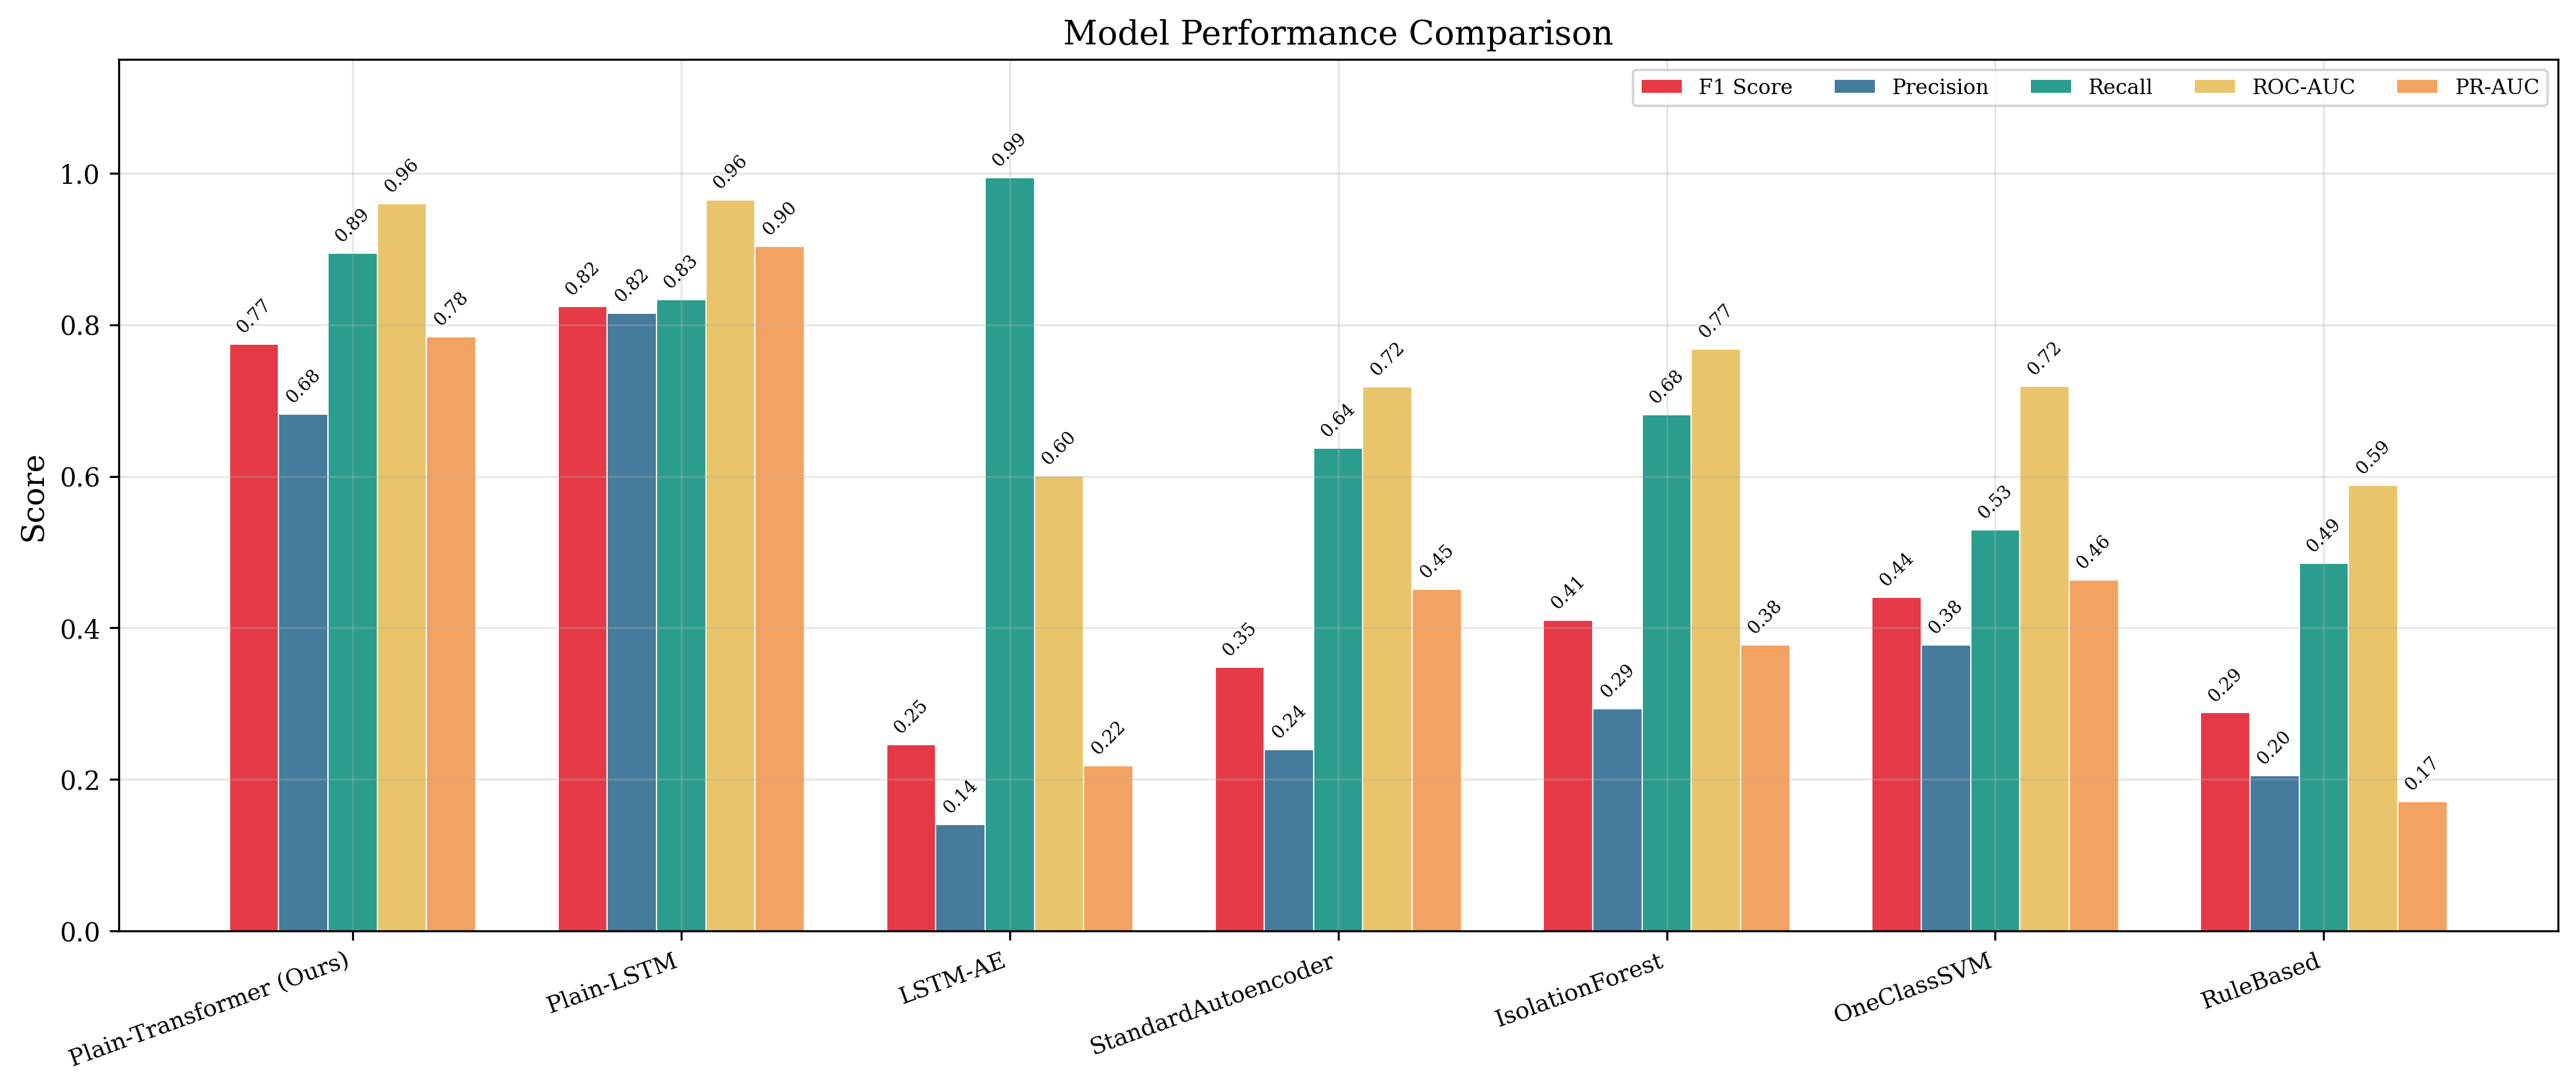
\includegraphics[width=\columnwidth]{model_comparison.png}
\caption{Side-by-side summary of all seven detectors on the four headline metrics: ROC-AUC, PR-AUC, F1, and Recall.}
\label{fig:modelcmp}
\end{figure}

\begin{figure}[htbp]
\centering
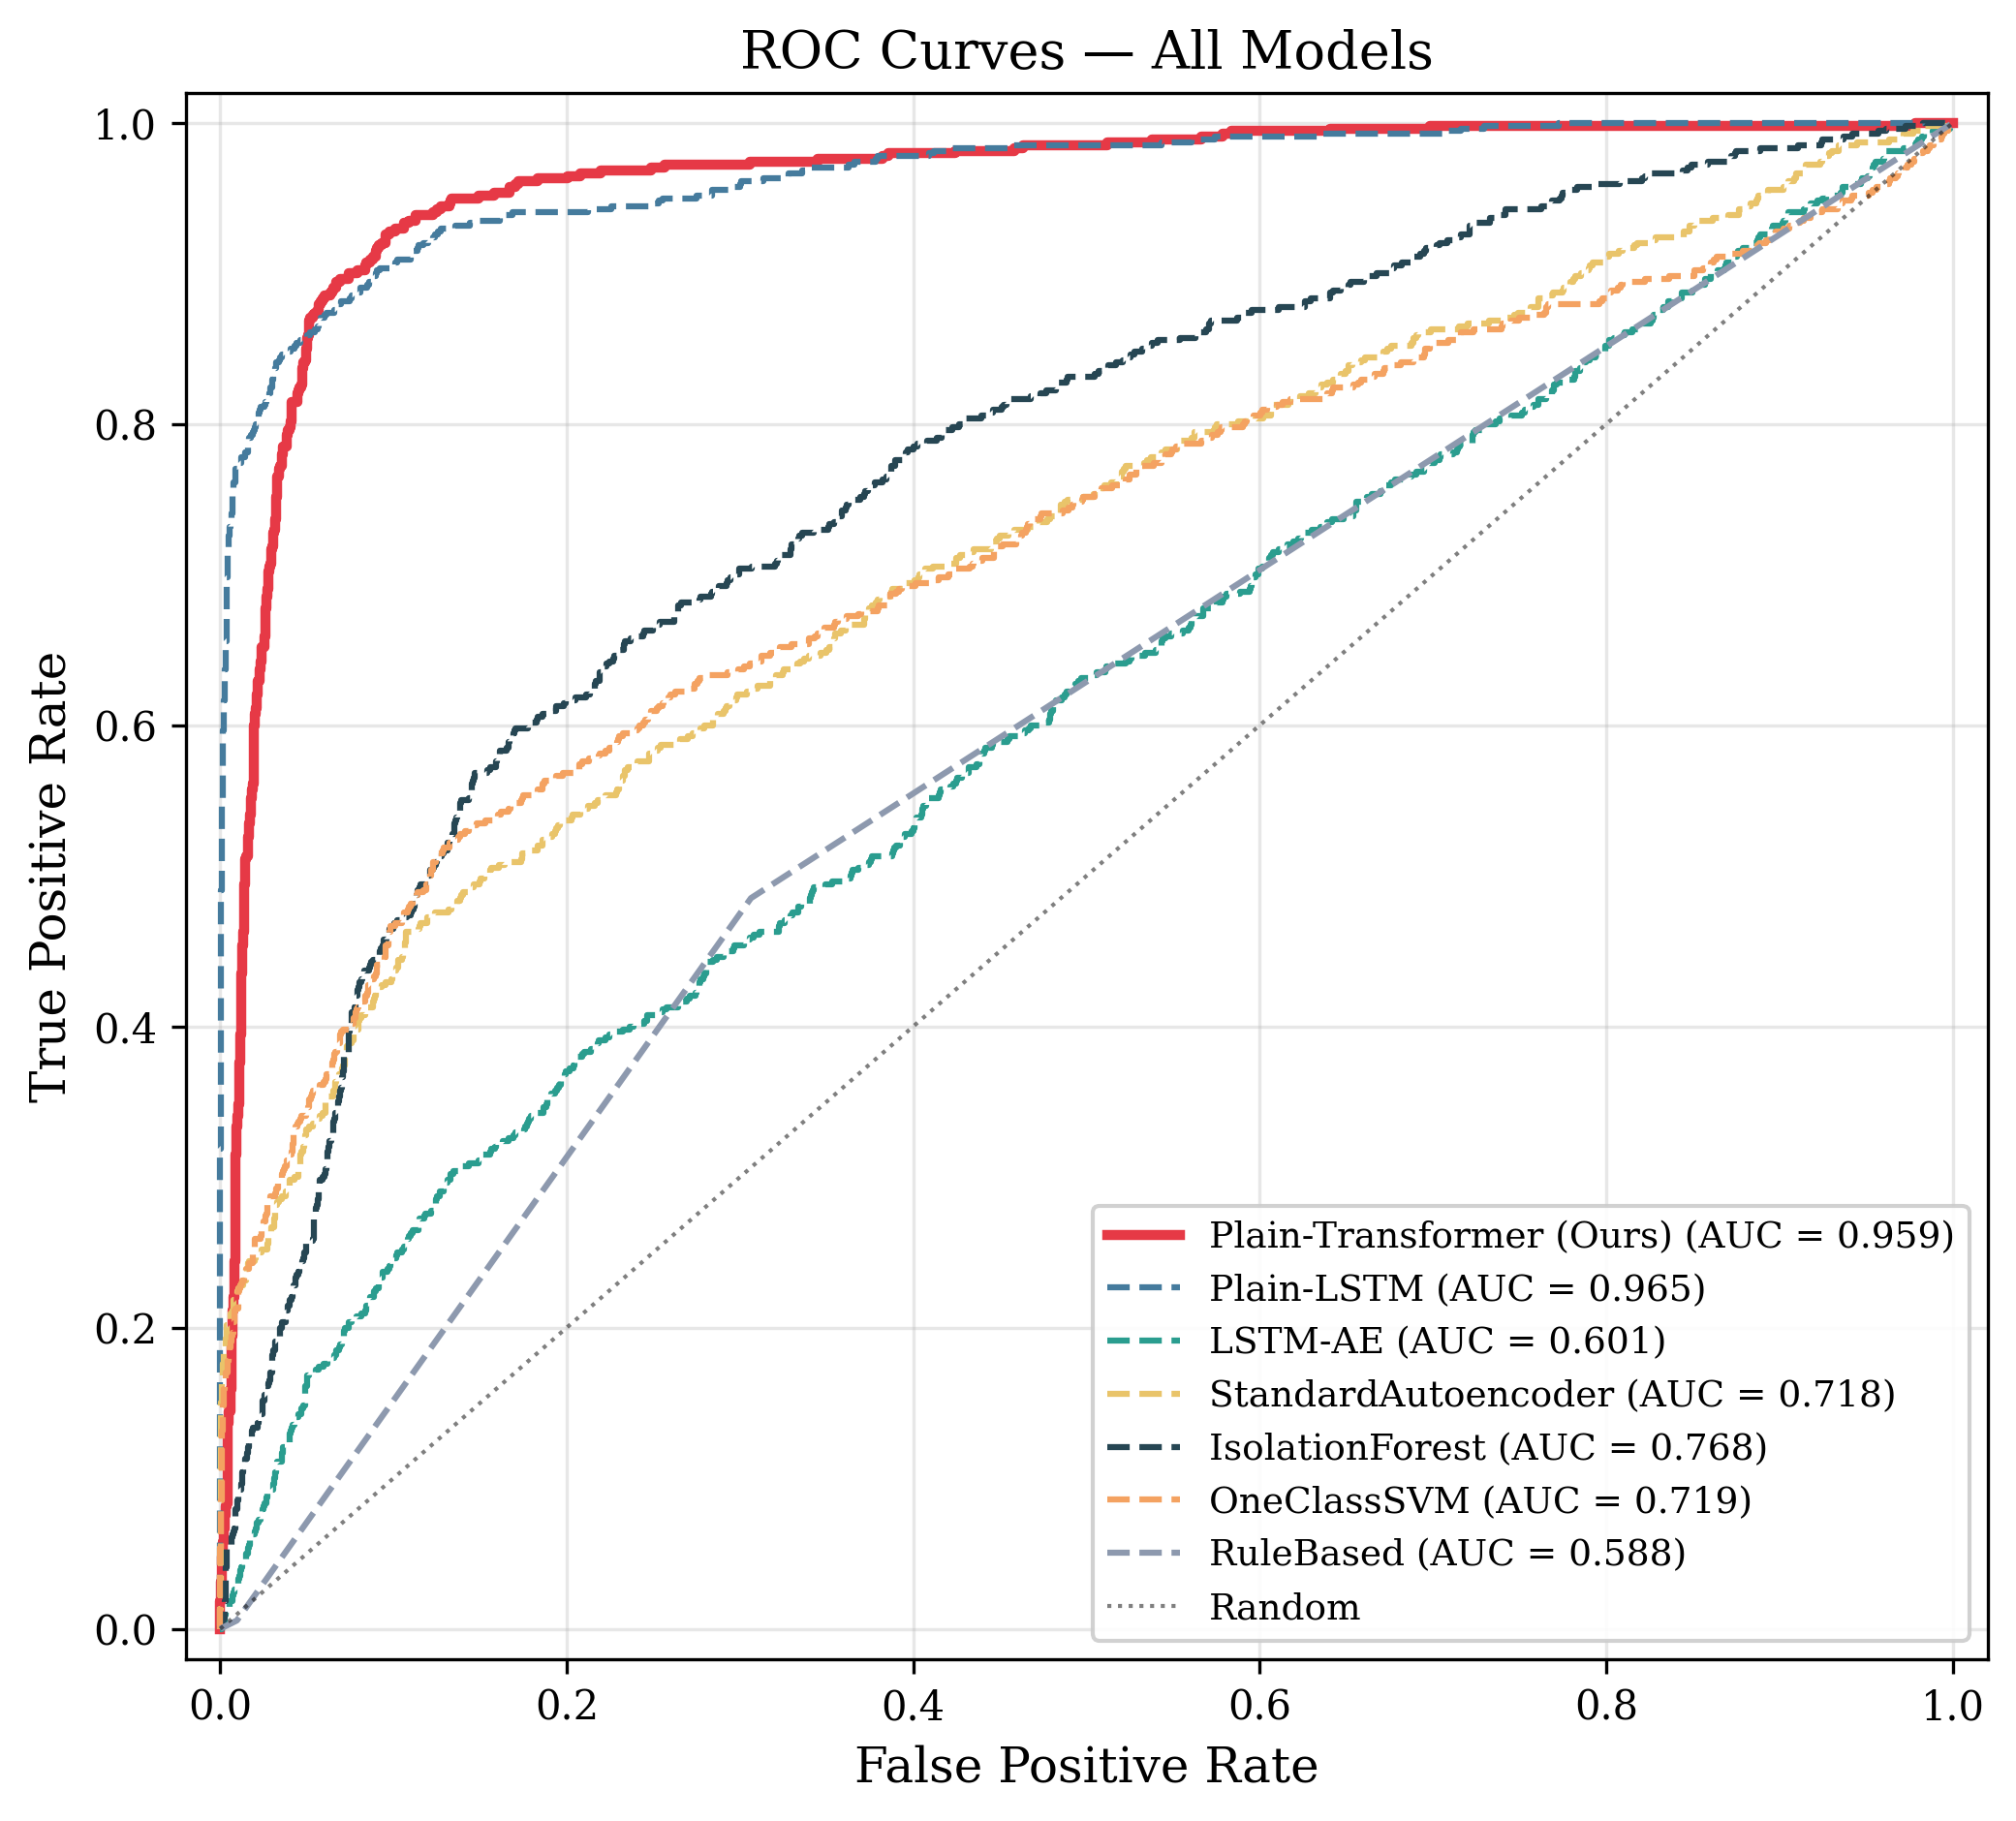
\includegraphics[width=\columnwidth]{roc_curves.png}
\caption{ROC curves on the held-out test split. Both personalised supervised sequence models (Transformer, BiLSTM) dominate; the self-supervised LSTM-AE underperforms the Standard-AE, which we attribute to the higher-capacity action-level representation being harder to reconstruct faithfully.}
\label{fig:roc}
\end{figure}

\begin{figure}[htbp]
\centering
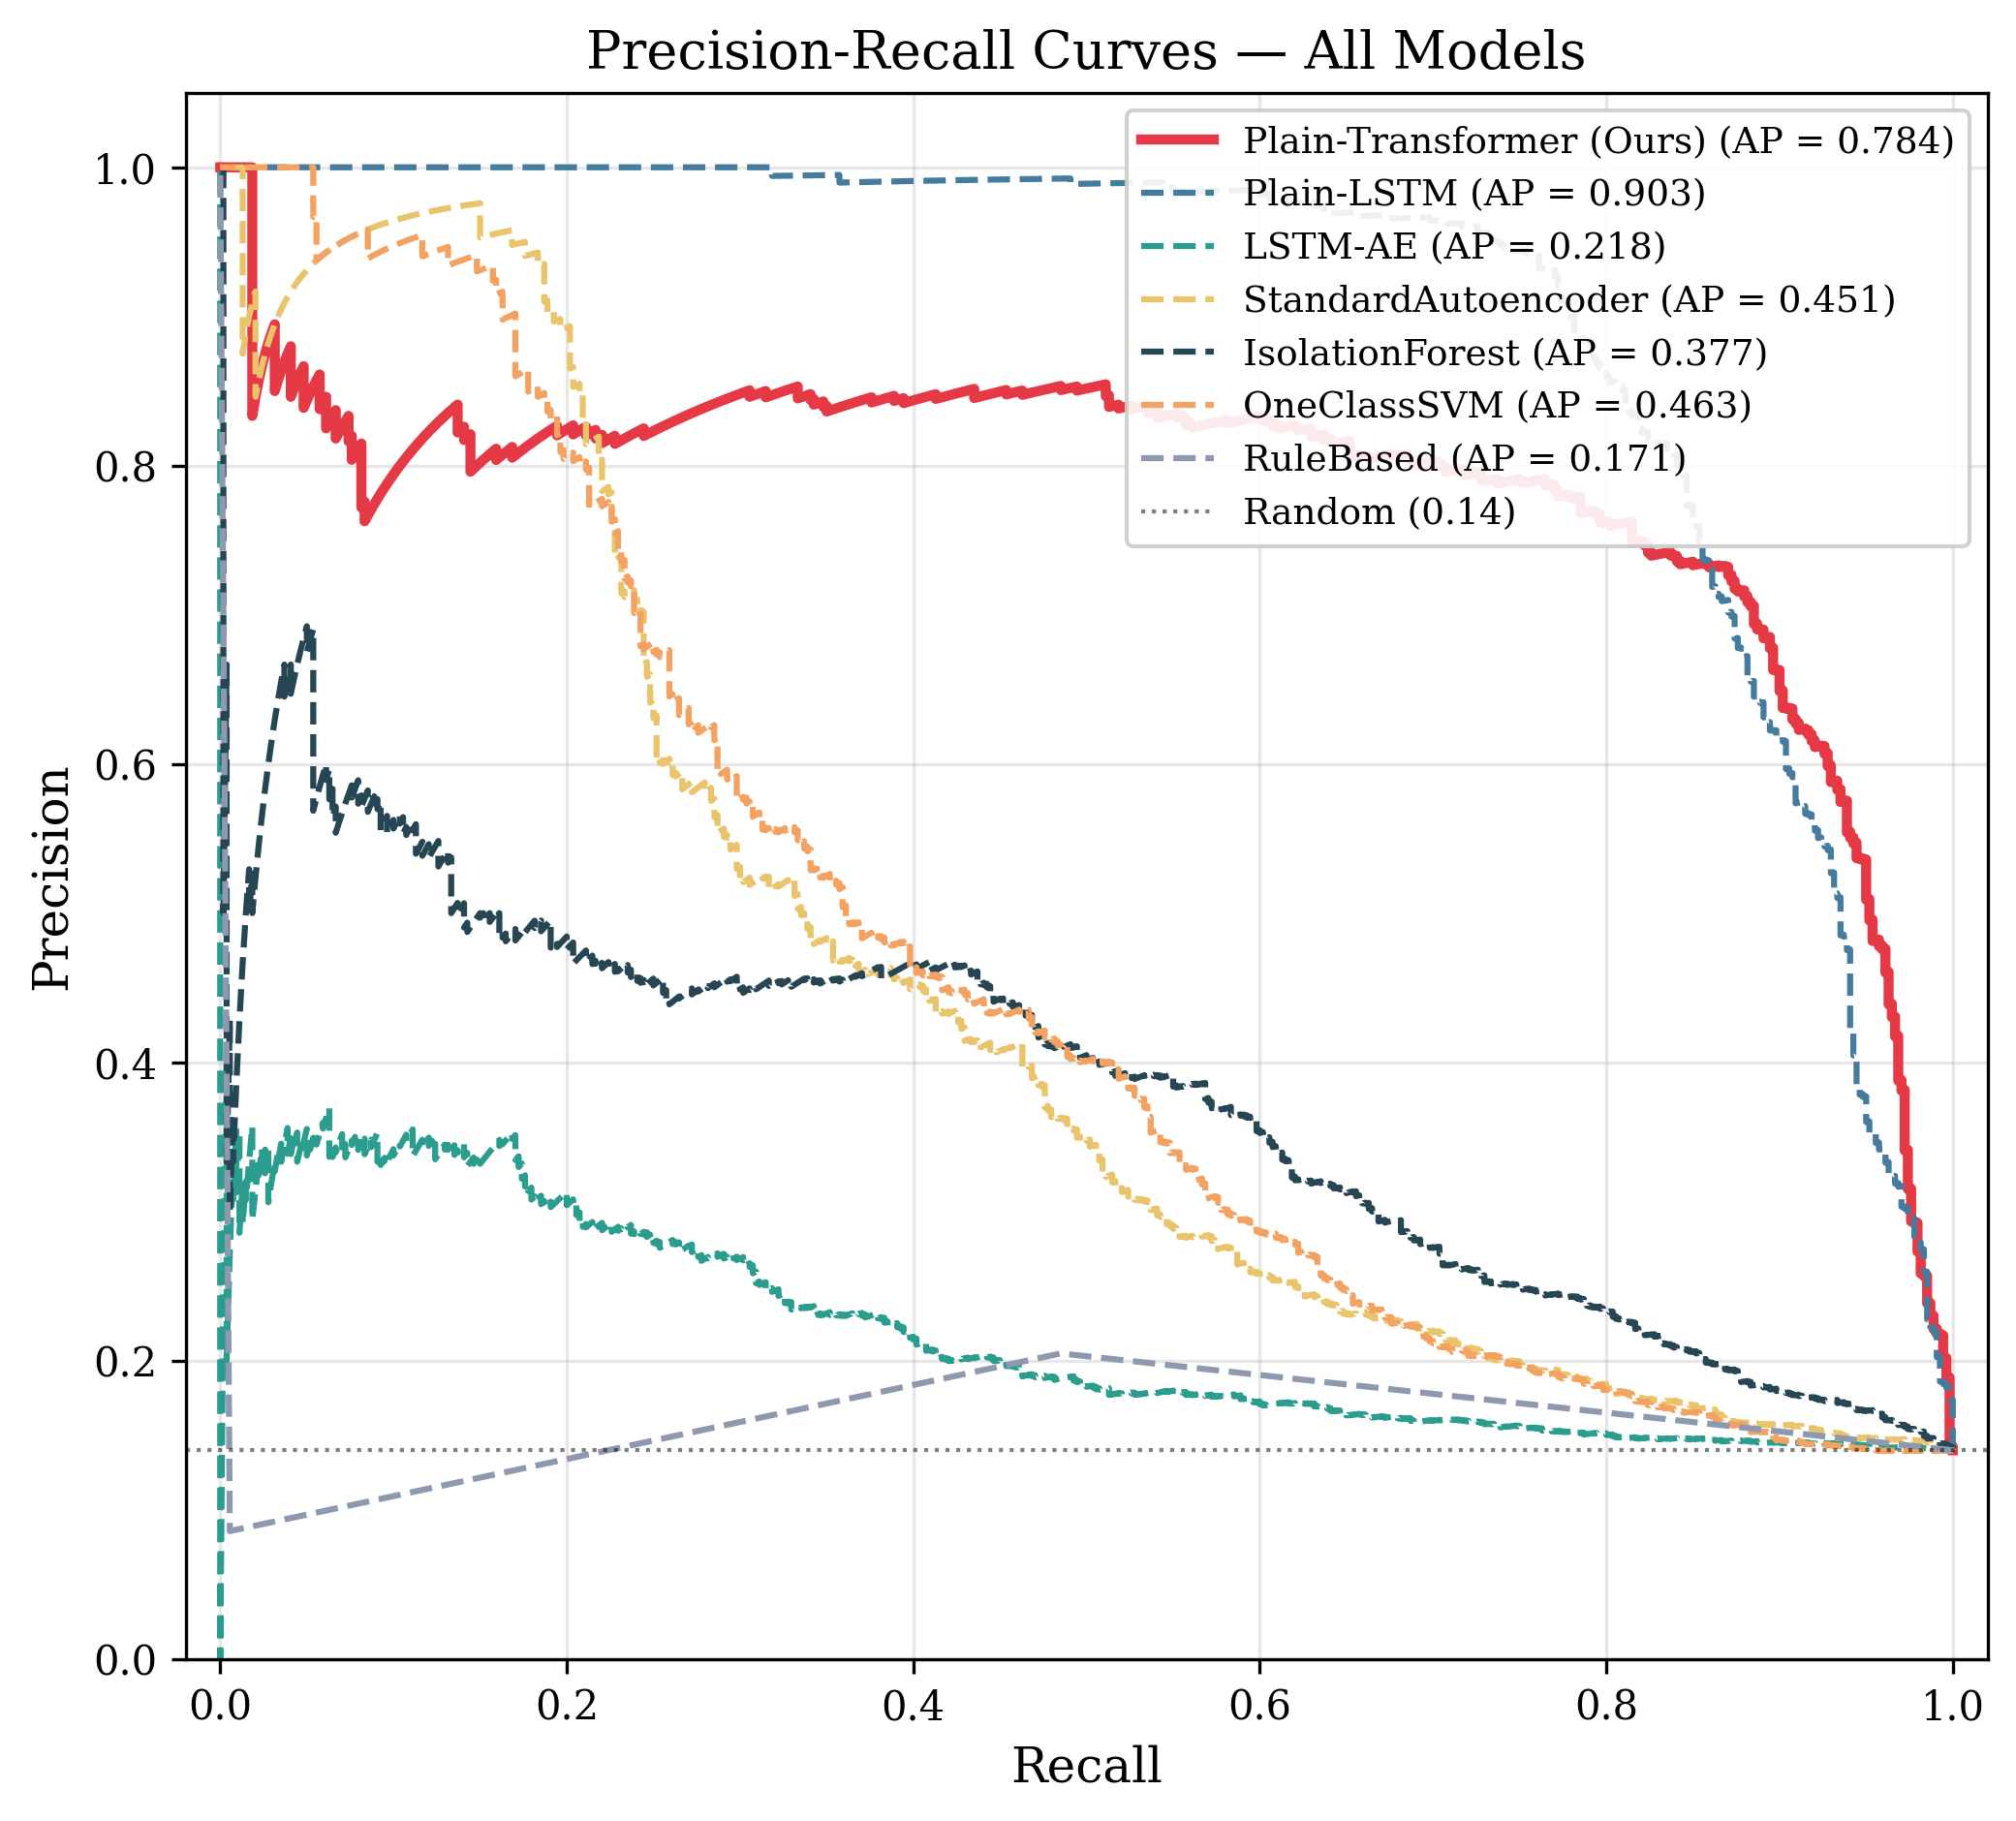
\includegraphics[width=\columnwidth]{pr_curves.png}
\caption{Precision-Recall curves. The personalised Transformer maintains a consistent lead over the personalised BiLSTM across the operating range, with the gap most visible in the high-recall regime where shortlisting tools operate.}
\label{fig:pr}
\end{figure}

\begin{figure}[htbp]
\centering
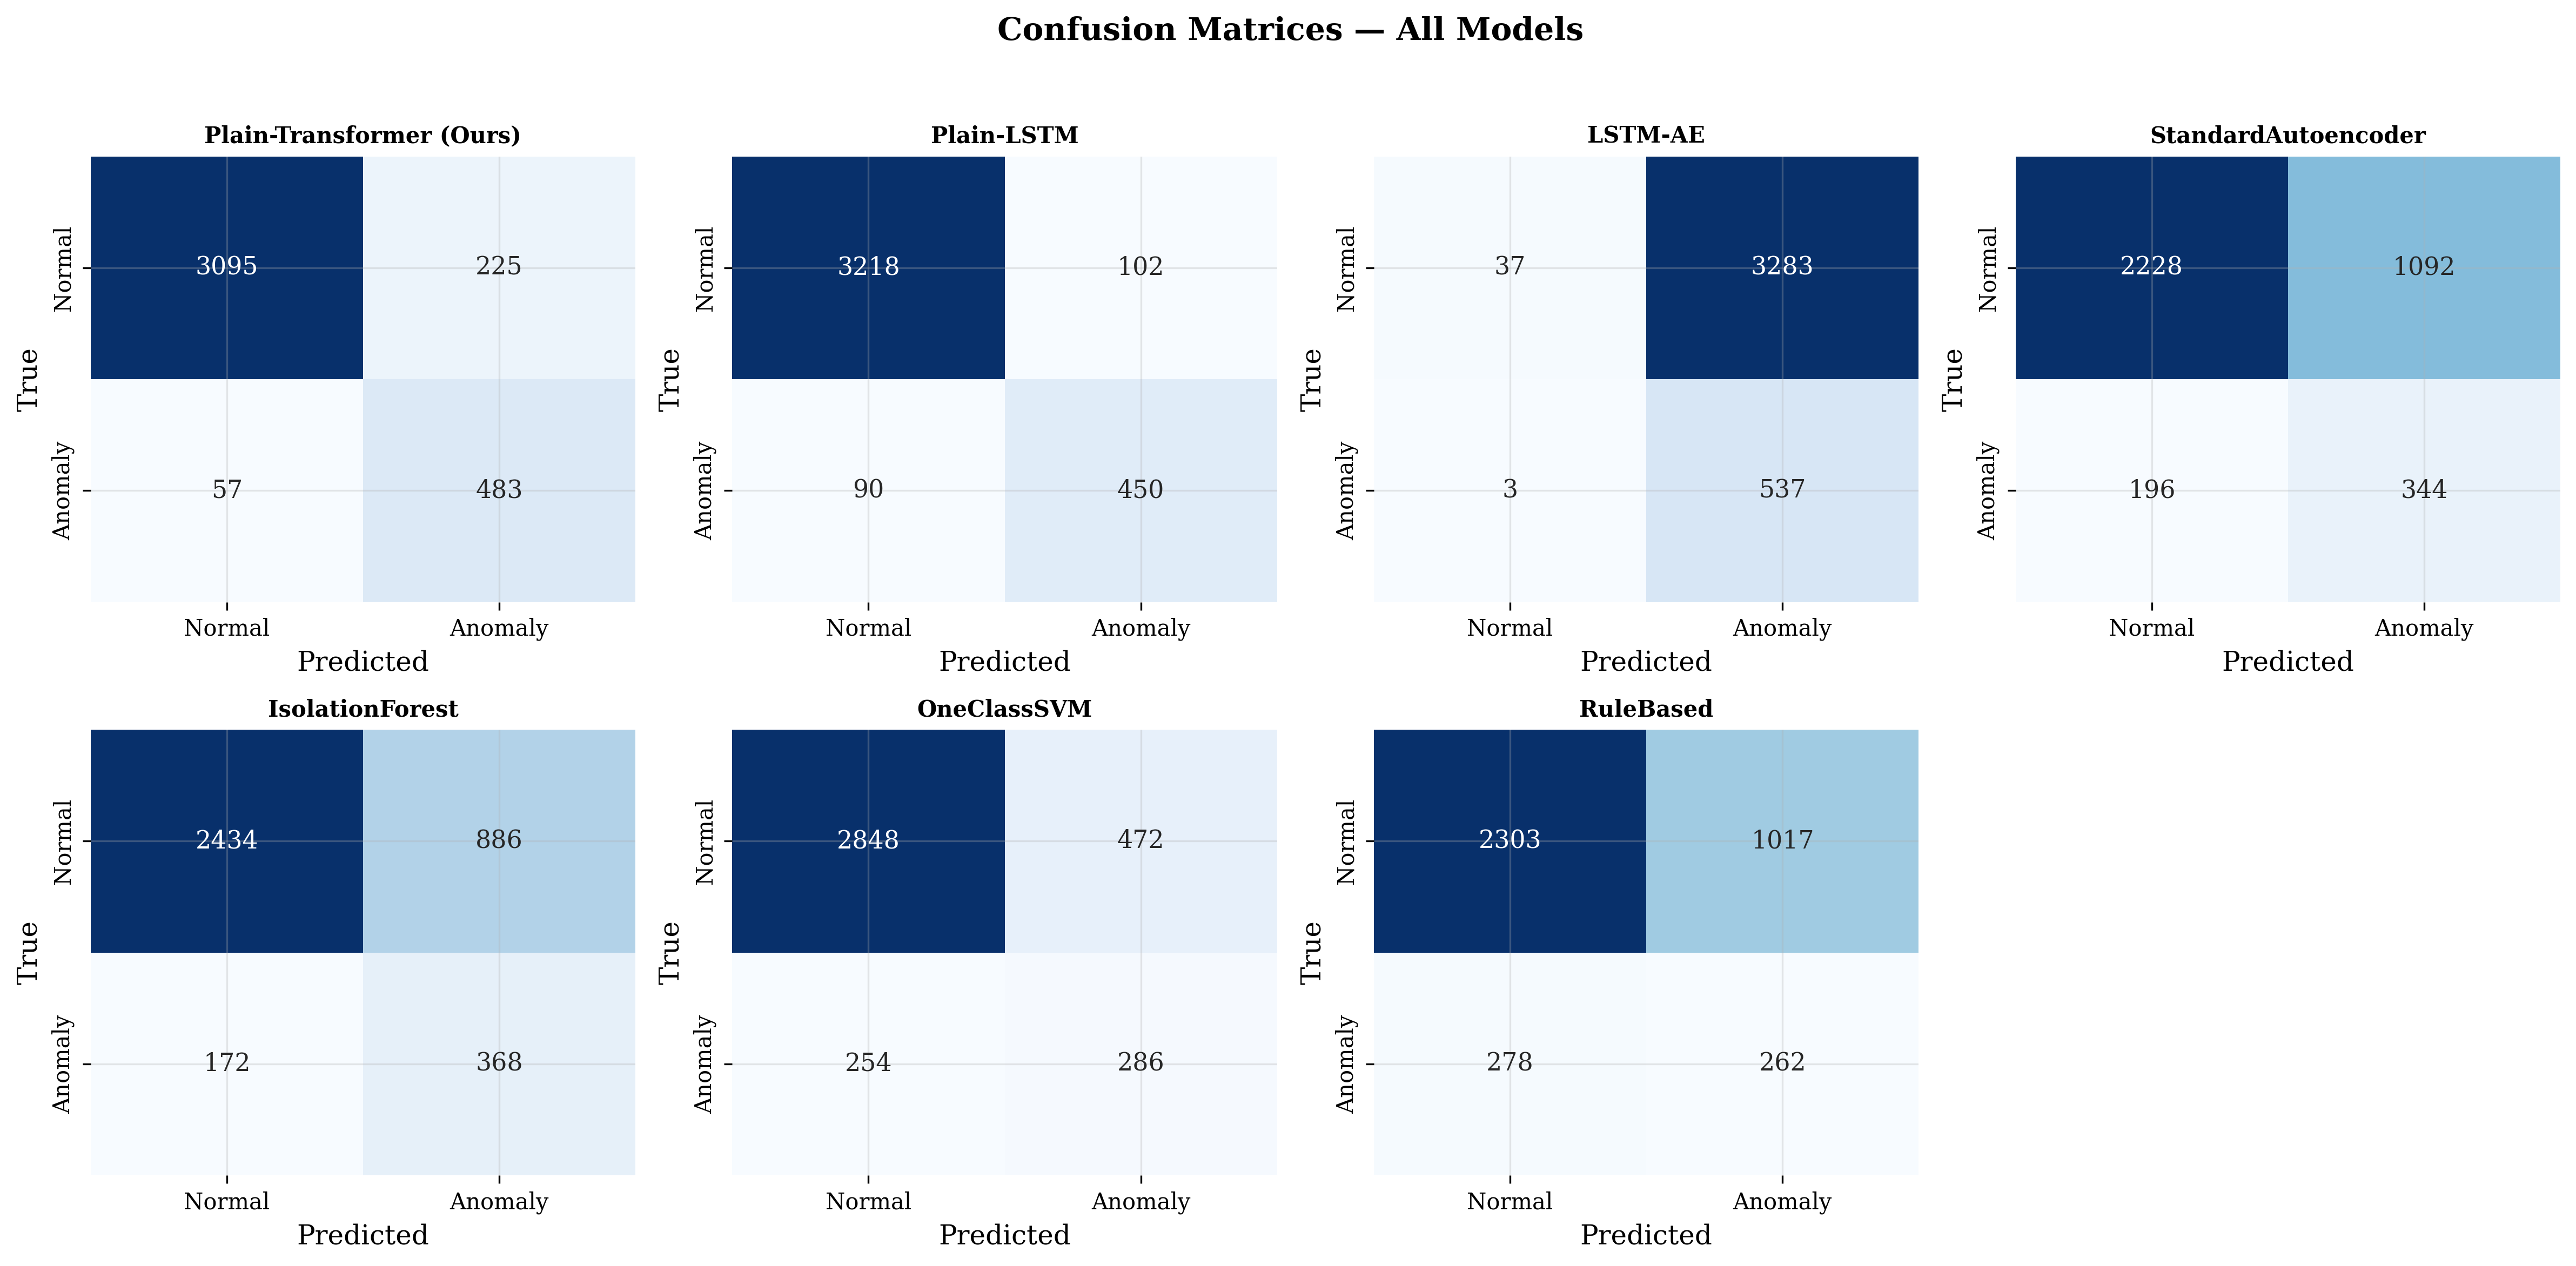
\includegraphics[width=\columnwidth]{confusion_matrices.png}
\caption{Confusion matrices at each model's tuned operating threshold. The Transformer trades a slightly higher false-positive count for a recall of $0.894$, consistent with its role as a shortlisting tool for instructor review.}
\label{fig:cm}
\end{figure}

\begin{figure}[htbp]
\centering
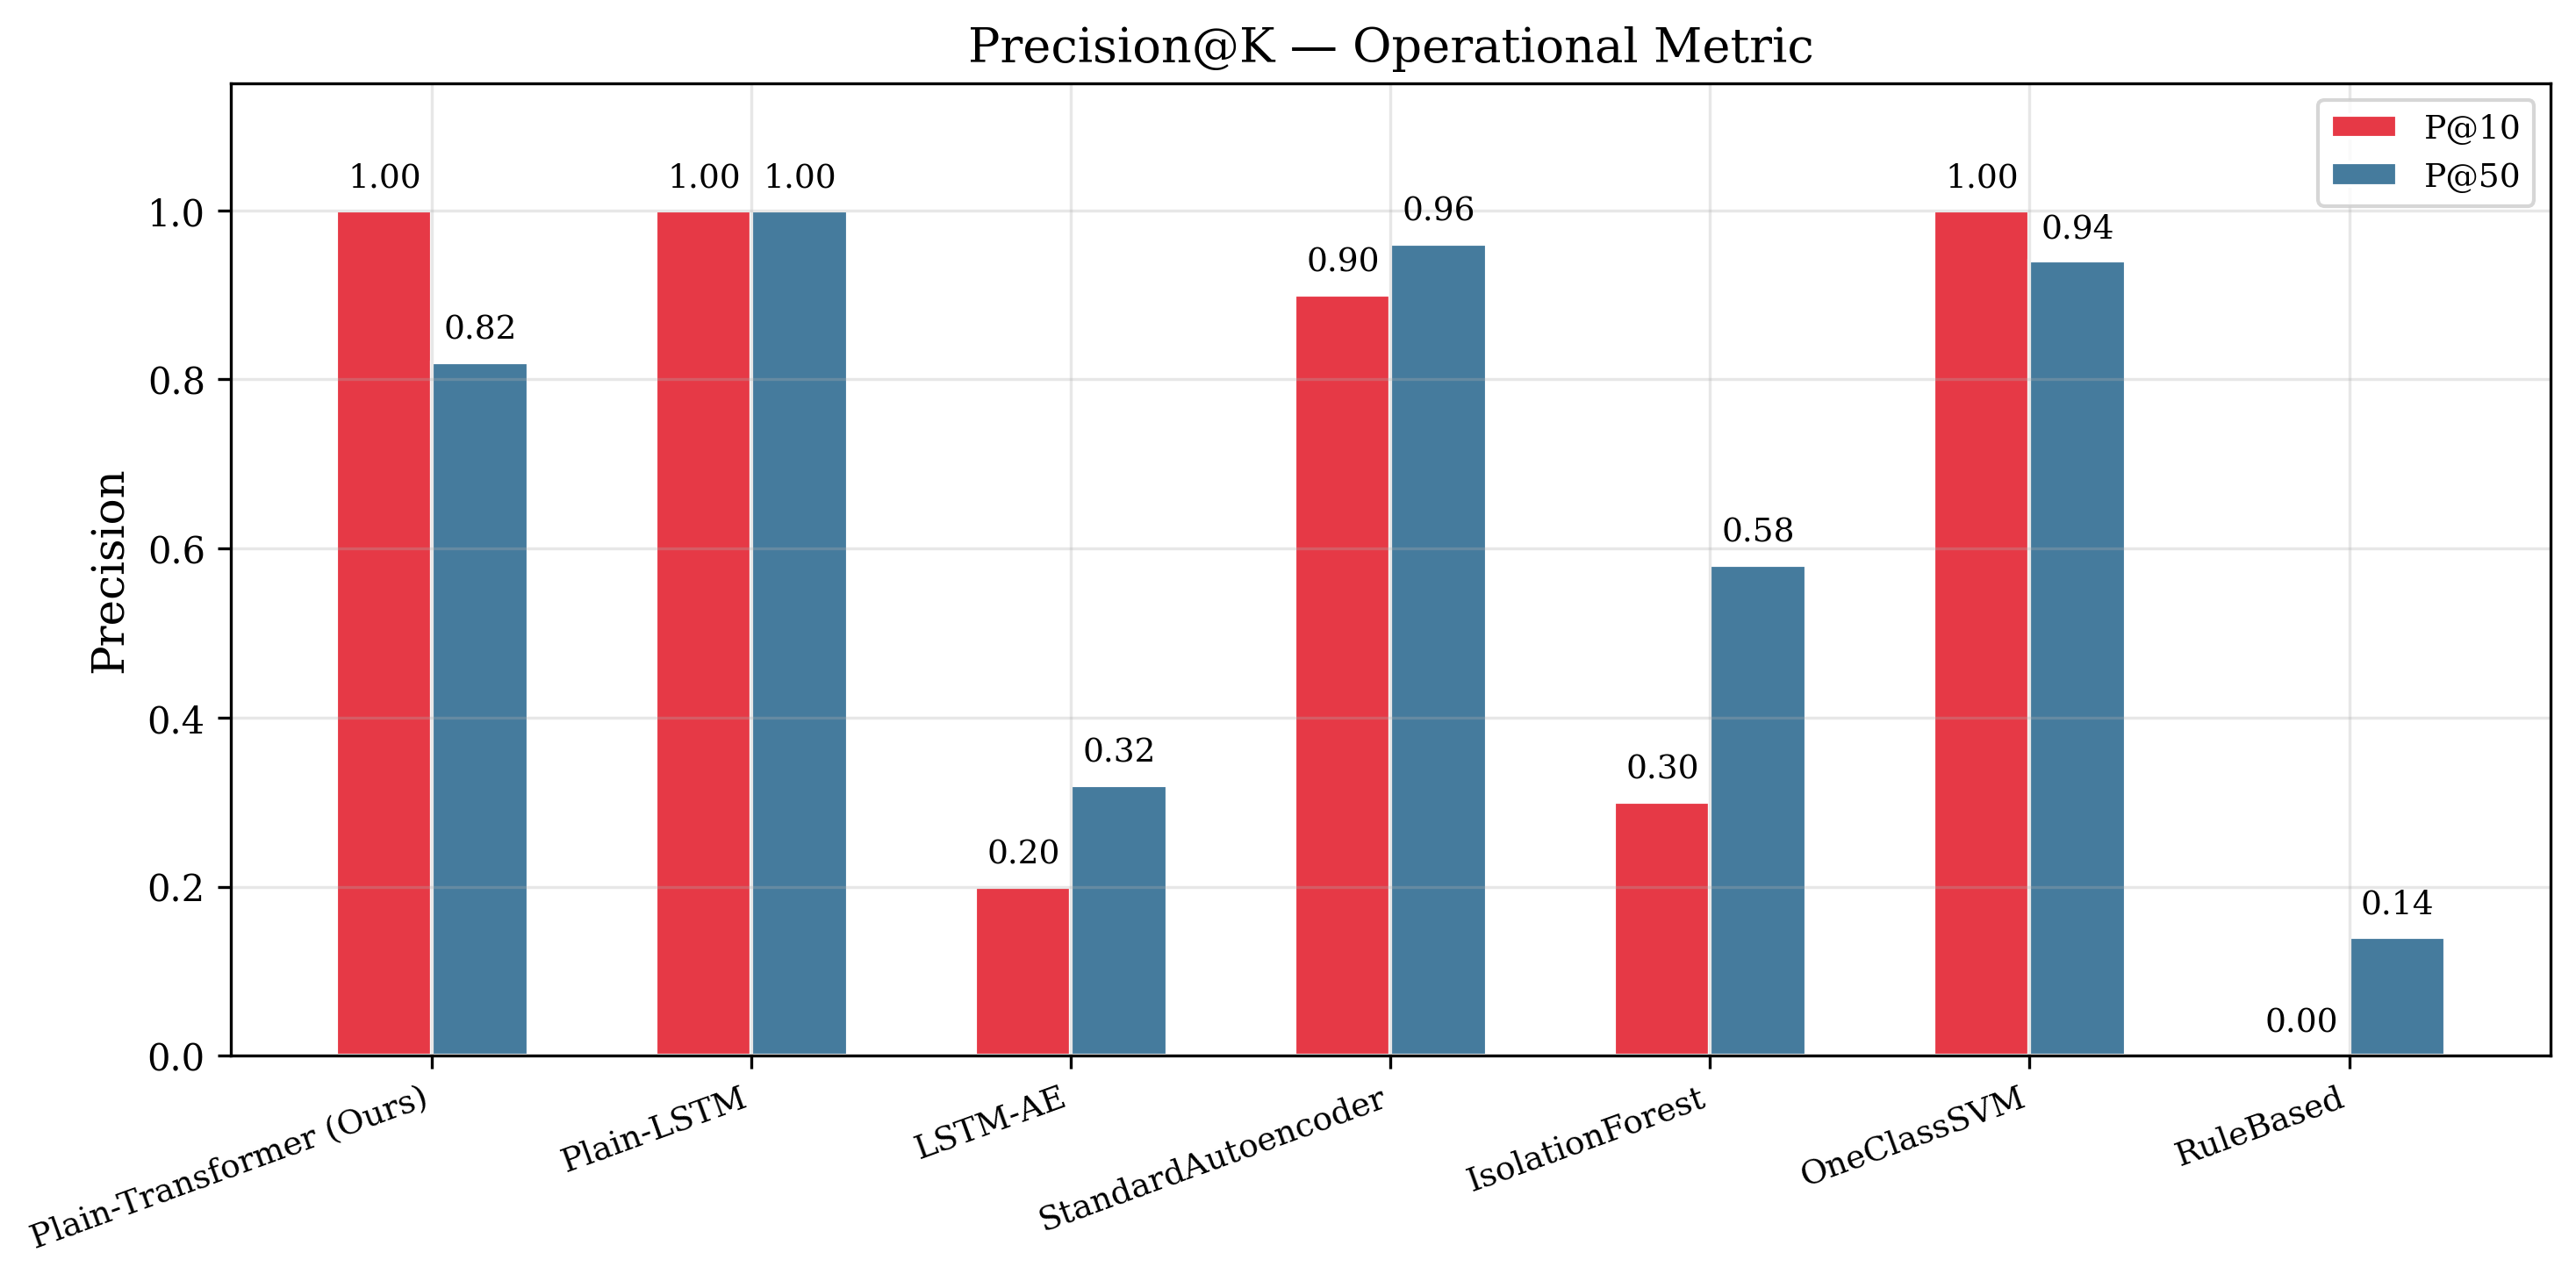
\includegraphics[width=\columnwidth]{precision_at_k.png}
\caption{Precision-at-$k$ curves. Both supervised models achieve perfect precision over the top-50 ranked sessions, operationally the most relevant regime for instructors who only review a shortlist.}
\label{fig:pk}
\end{figure}

\begin{figure}[htbp]
\centering
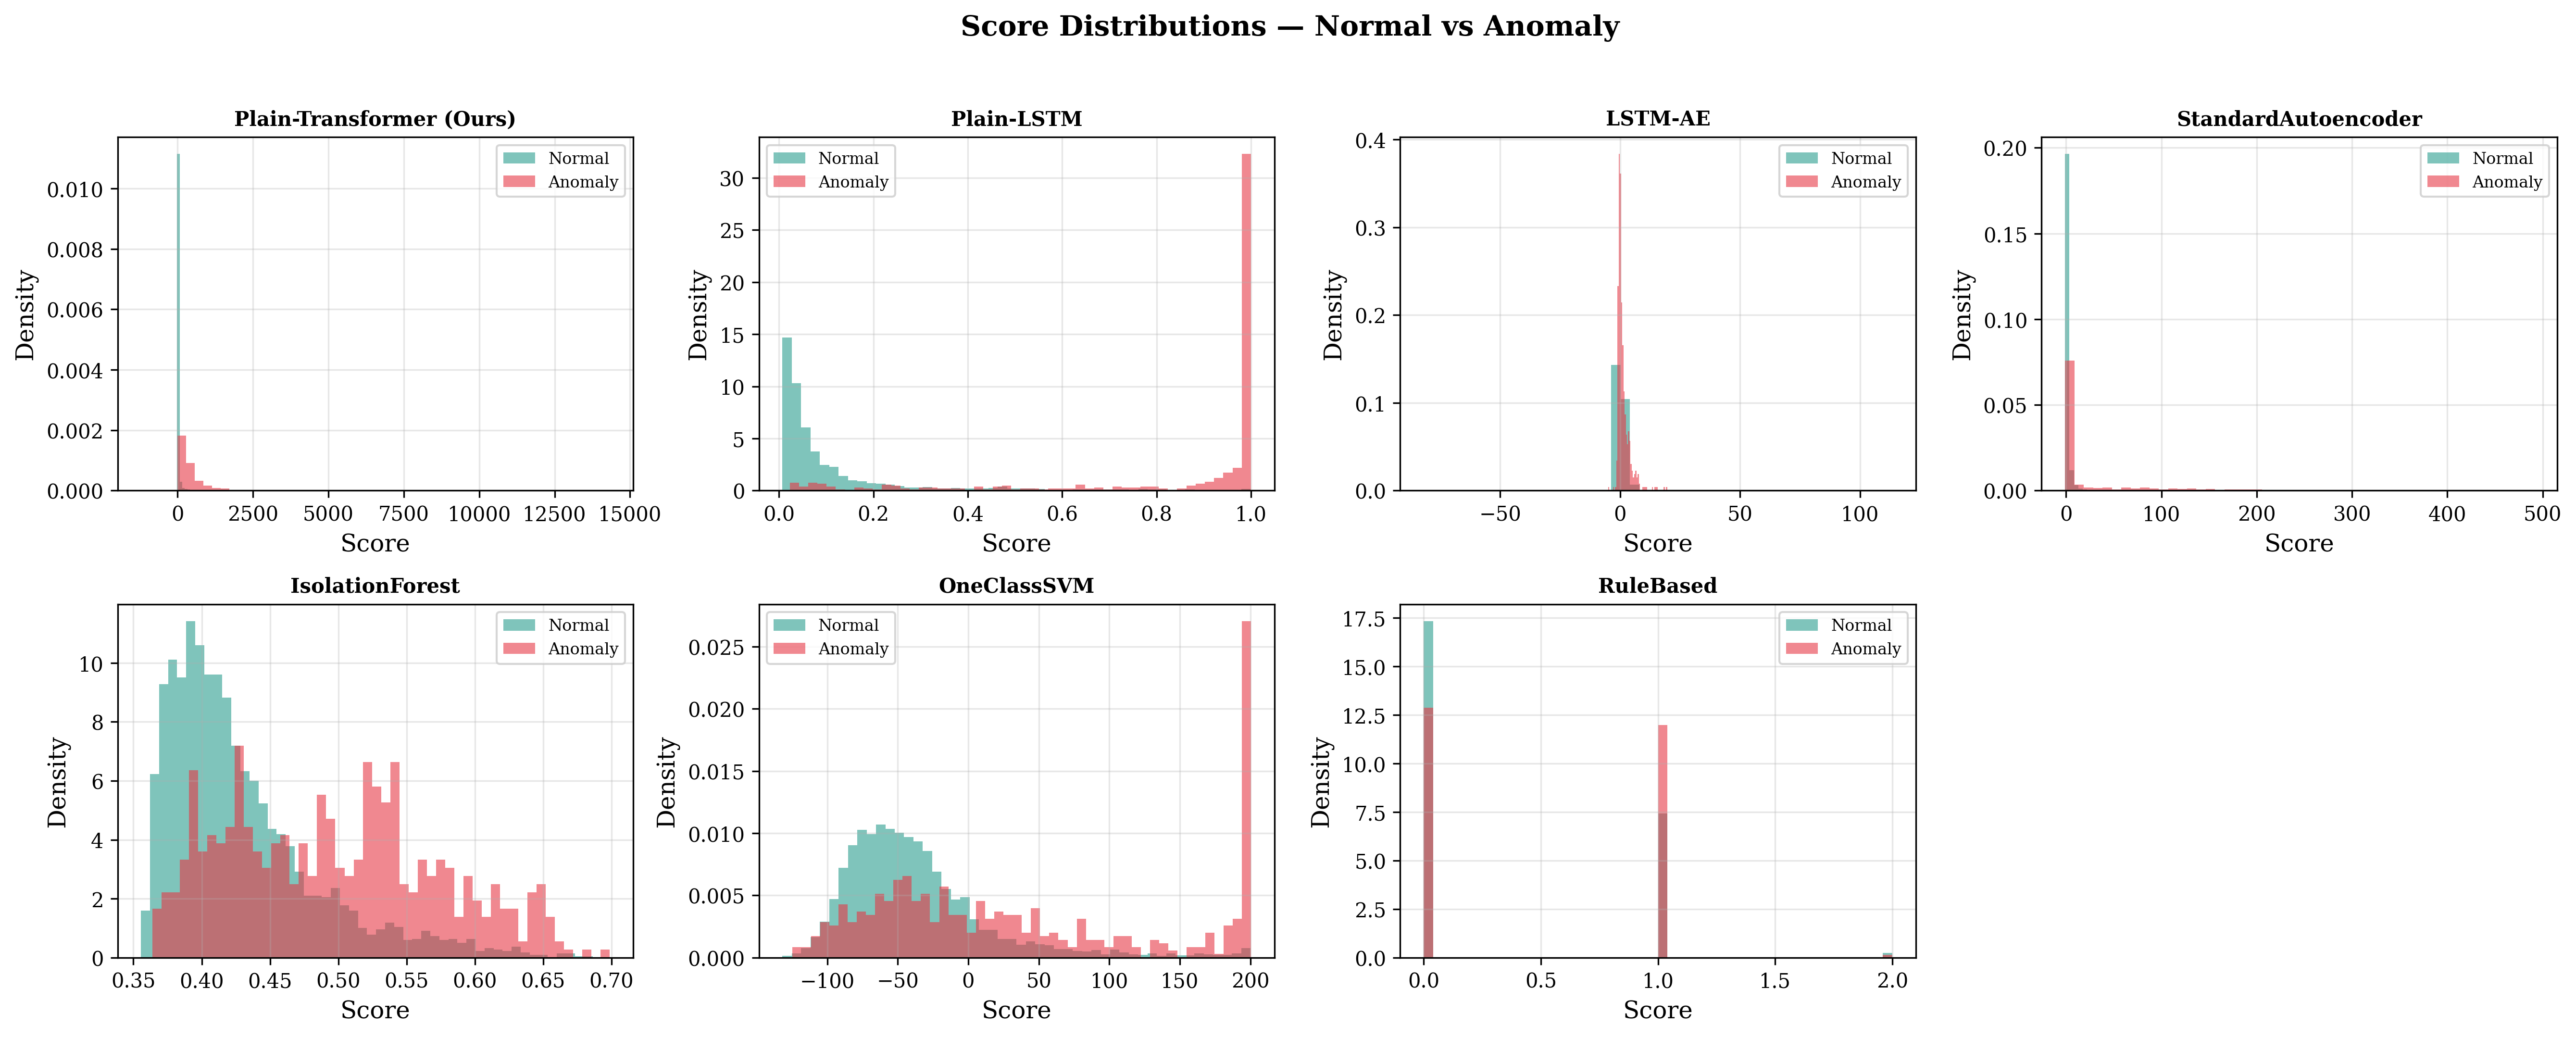
\includegraphics[width=\columnwidth]{score_distributions.png}
\caption{Anomaly-score distributions for normal vs anomalous sessions. The supervised sequence models produce clean bimodal separations; the LSTM-AE reconstruction scores overlap substantially, consistent with its lower ROC-AUC.}
\label{fig:scores}
\end{figure}

A few observations stand out from Table~\ref{tab:main_results}. (i) The two supervised sequence models (Transformer, BiLSTM) sit clearly above all unsupervised baselines, with ROC-AUC around $0.95$--$0.96$ versus $0.60$--$0.77$ for the rest. (ii) Across every shared metric, the personalised Transformer beats the personalised BiLSTM by a small but consistent margin: $+0.008$ ROC-AUC, $+0.013$ PR-AUC, $+0.049$ F1, $+0.058$ Precision, and $+0.025$ Recall, with bootstrap CIs that overlap only marginally on ROC-AUC and PR-AUC. The Transformer is also the only sequence model that holds perfect P@10. (iii) Both supervised models trade some precision for recall under the personalised score, which is the right operating-point bias for an instructor-review tool that surfaces a shortlist of suspicious sessions. (iv) The LSTM autoencoder collapses on action-level inputs (ROC-AUC $0.60$, F1 $0.25$): reconstructing $100\!\times\!10$ tensors is a much harder objective than emitting a single anomaly logit, and the bottleneck reconstructs rare-but-normal and rare-but-anomalous patterns about equally well. Standard-AE on session-level features and Isolation Forest both outperform it. (v) Rule-Based is the floor, confirming that hand-tuned thresholds cannot keep up with per-student variability.

\subsection{Ablation: What Does the Transformer Actually Buy?}
\label{sec:ablation}
The Transformer and BiLSTM classifiers share an identical training pipeline: the same GAN-augmented labels, the same action-level input tensor, the same masked-mean pooling, the same MLP head, \emph{and} the same inference-time per-student blending step (Equation~$4$). Their gap in Table~\ref{tab:main_results} is therefore due solely to the \emph{sequence encoder} (self-attention vs.\ stacked recurrence), summarised in Table~\ref{tab:ablation_arch}. The lift from attention is small but pointing the right way on every metric.

\begin{table}[htbp]
\caption{Supervised-architecture ablation on the full pipeline (15K students, GAN-augmented training): Transformer vs.\ BiLSTM, holding the training recipe \emph{and} the inference-time personalised blending fixed. The encoder is the only variable.}
\label{tab:ablation_arch}
\centering
\small
\begin{tabular}{lcccc}
\toprule
\textbf{Encoder} & \textbf{ROC-AUC} & \textbf{PR-AUC} & \textbf{F1} & \textbf{Recall} \\
\midrule
BiLSTM (personalised)               & $0.951$ & $0.771$ & $0.725$ & $0.869$ \\
\textbf{Transformer (personalised)} & $\mathbf{0.959}$ & $\mathbf{0.784}$ & $\mathbf{0.774}$ & $\mathbf{0.894}$ \\
\midrule
$\Delta$ (TF $-$ BiLSTM)            & $+0.008$ & $+0.013$ & $+0.049$ & $+0.025$ \\
\bottomrule
\end{tabular}
\end{table}

\paragraph{GAN-vs-rule-only synthesis (anomaly-source ablation).} A reviewer concern raised against earlier drafts of this work was that the role of the GAN augmentation step was asserted but not measured. We address this directly with a controlled comparison run on a $3$K-student subset of EdNet (held fixed across both arms), in which the only varied component is \texttt{synthetic\_method}: \emph{rule-only} (the literature-grounded generators of Section~\ref{subsec:datasets}) versus \emph{GAN-augmented} (the same rules used as training seed for the conditional GAN, with $50\%$ of training-split anomalies replaced by GAN samples). Both arms use the same Transformer hyperparameters, the same chronological per-student split, and the same threshold-selection procedure. Table~\ref{tab:ablation_gan} reports the result.

\begin{table}[htbp]
\caption{Anomaly-source ablation on the held-out test split (3K-student subset). Only the source of training-time anomalies differs; everything else is held fixed.}
\label{tab:ablation_gan}
\centering
\small
\begin{tabular}{lcccc}
\toprule
\textbf{Anomaly source} & \textbf{ROC-AUC} & \textbf{PR-AUC} & \textbf{F1} & \textbf{Recall} \\
\midrule
Rule-only                       & $0.951$ & $0.892$ & $0.829$ & $0.776$ \\
GAN-augmented (default)         & $0.950$ & $0.891$ & $0.819$ & $0.776$ \\
\midrule
$\Delta$ (GAN $-$ rule)         & $-0.001$ & $-0.001$ & $-0.010$ & $0.000$ \\
\bottomrule
\end{tabular}
\end{table}

The two arms are statistically indistinguishable on detection metrics. We retain GAN augmentation as the default for two reasons that the metrics in Table~\ref{tab:ablation_gan} cannot directly express: (i) GAN samples introduce within-family distributional variation beyond the fixed parameter ranges of the rule generators, which is the kind of regularisation we want when test-time anomalies may not look exactly like the training templates; and (ii) reporting only the rule-only number would understate how synthetic the evaluation is, because the test split itself is rule-based. The honest reading of Table~\ref{tab:ablation_gan} is that, at the scale of this evaluation, the GAN does not deliver a measurable gain; its role should be understood as guarding against template overfitting, with empirical evidence for that claim deferred to a future cross-distribution study.

\paragraph{Where the gains actually come from.} Reading Tables~\ref{tab:main_results}, \ref{tab:ablation_arch}, and~\ref{tab:ablation_gan} together, the contributions to the supervised models' lead can be ranked: the largest single jump is the \emph{self-supervised $\to$ supervised} paradigm shift on action-level inputs (the supervised models reach ROC-AUC $\sim 0.95$ where the LSTM autoencoder collapses to $0.60$); next is the \emph{population $\to$ personalised} inference-time scoring (Equation~$4$), which is what makes the title's ``personalised drift'' framing hold for the main detector and not just the LSTM-AE baseline; the encoder structure (recurrence vs.\ attention) is a small but consistent positive on every metric ($+0.008$--$+0.049$); and the anomaly source (rule vs.\ GAN) does not move the metric here at all. The framework's headline number is therefore best read as a property of \emph{action-level representation $+$ supervised training $+$ personalised inference}, with the Transformer encoder providing the additional consistency margin.

\subsection{Per-Anomaly-Family Performance}
\label{sec:per_family}
Because the rule-based generators expose the family of each injected anomaly, we can break the Transformer's recall down by family rather than reporting a single aggregate. Table~\ref{tab:per_family} shows the result.

\begin{table}[htbp]
\caption{Per-anomaly-family detection performance for the Transformer detector. ``ROC-AUC vs.\ normals'' is computed by pooling each family's anomalies with all clean test sessions, so the columns are not directly summable.}
\label{tab:per_family}
\centering
\small
\begin{tabular}{lccc}
\toprule
\textbf{Family} & \textbf{$n$} & \textbf{Recall} & \textbf{ROC-AUC vs.\ normals} \\
\midrule
answer\_copying                 & $116$ & $0.983$ & $0.981$ \\
partial\_session                & $99$  & $0.970$ & $0.975$ \\
lookup\_behavior                & $106$ & $0.934$ & $0.972$ \\
panic\_compression              & $103$ & $0.796$ & $0.931$ \\
pre\_known\_answers             & $116$ & $0.793$ & $0.939$ \\
\bottomrule
\end{tabular}
\end{table}

The detector is strongest on families with the largest local timing signature (\emph{answer\_copying}, \emph{partial\_session}, \emph{lookup\_behavior}: recall $\geq 0.93$) and weakest on the two whole-session compression families, \emph{panic\_compression} and \emph{pre\_known\_answers}, where the perturbation is more uniform across the action sequence and easier to confuse with a fast-but-honest examinee. This breakdown is consistent with the role of self-attention: distributed local signals are easier for attention to localise than uniform global rescalings, which look more like a baseline shift.

\subsection{Cold-Start: Performance by Number of Prior Sessions}
\label{sec:cold_start}
A central question for any personalised system is whether performance degrades when a student has little or no history. We bucket the test split by the number of prior (training) sessions for the corresponding student and report the Transformer's metrics within each bucket in Table~\ref{tab:cold_start}.

\begin{table}[htbp]
\caption{Transformer detection performance bucketed by the number of prior training sessions for the test student. The personalised blending weight $\lambda_u$ ranges from $\le 0.4$ in the leftmost bucket to $1.0$ in the rightmost.}
\label{tab:cold_start}
\centering
\small
\begin{tabular}{lcccc}
\toprule
\textbf{Prior sessions} & \textbf{$n_{\text{test}}$} & \textbf{ROC-AUC} & \textbf{F1} & \textbf{Recall} \\
\midrule
$1$--$2$  & $196$  & $0.954$ & $0.694$ & $0.926$ \\
$3$--$4$  & $396$  & $0.960$ & $0.724$ & $0.939$ \\
$\geq 5$  & $3{,}268$ & $0.960$ & $0.786$ & $0.888$ \\
\bottomrule
\end{tabular}
\end{table}

ROC-AUC is essentially flat across buckets ($0.954$--$0.960$), which is the property the $\lambda_u$ blend was designed to deliver: when $n_u$ is small the detector smoothly defers to the population baseline, so cold-start examinees are not penalised. F1 is lower in the cold-start buckets, but the recall in those buckets is actually higher than in the warm bucket; this is the precision component dropping under thinner data, not a recall failure. In a deployed system the obvious mitigation is to flag the first one or two sessions of any student with lower confidence, regardless of score.

\subsection{Top False Positives and False Negatives}
\label{sec:errors}
Table~\ref{tab:fp_fn} lists the five highest-scoring false positives and the five lowest-scoring (i.e., most confident) false negatives produced by the Transformer detector on the held-out test split. Two patterns are worth noting. First, the top false positives are concentrated on a small number of distinct students (e.g., \texttt{u261015} appears twice, \texttt{u261200} once), suggesting these are individuals whose \emph{normal} behaviour genuinely looks anomalous against the population baseline. The personalised blend pulls their scores toward zero but not always enough; deepening per-student calibration with more sessions per student is the natural fix. Second, the top false negatives are dominated by the two whole-session compression families (\emph{pre\_known\_answers}, \emph{panic\_compression}), which is consistent with the per-family breakdown in Table~\ref{tab:per_family}. These are anomalies whose perturbation is uniform across the sequence and therefore look most like a faster-than-usual but otherwise normal session.

\begin{table}[htbp]
\caption{Top false positives and false negatives for the Transformer on the held-out test split. ``Family'' is \emph{normal} for genuine clean sessions misclassified as anomalous, and the synthetic family for missed anomalies.}
\label{tab:fp_fn}
\centering
\small
\begin{tabular}{lll}
\toprule
\textbf{Rank} & \textbf{False positives (family / student)} & \textbf{False negatives (family / student)} \\
\midrule
1 & normal / u261015          & panic\_compression / u11304 \\
2 & normal / u261015          & partial\_session / u1802 \\
3 & normal / u275316          & pre\_known\_answers / u3380 \\
4 & normal / u283084          & pre\_known\_answers / u280770 \\
5 & normal / u3024            & panic\_compression / u1786 \\
\bottomrule
\end{tabular}
\end{table}

\subsection{Fairness Calibration: Mechanism Validation}
Table ~\ref{tab:fairness_results} reports demographic-parity and equalized-odds metrics for the Transformer detector, before and after per-group threshold calibration, across all four sensitive attributes. It is important to note that this evaluation constitutes validation of the calibration mechanism and not an empirical demonstration of fairness on naturally occurring demographic variation. Because EdNet-2 contains no demographic attributes, so synthetic samples were assigned from OULAD distributions and small controlled behavioural perturbations were manually introduced on per-group basis to specifically create calibration signal. The results below confirm that the post-hoc $\alpha$-calibration formula correctly removes those introduced disparities; they do not speak to whether disparities would exist or be correctable on a real exam situation with genuine demographic-behavioral correlations.

\begin{table}[htbp]
\caption{Fairness metrics for the Transformer detector, before and after per-group threshold calibration. DPR targets $\geq 0.80$; EOD targets $\leq 0.10$.}
\label{tab:fairness_results}
\centering
\small
\begin{tabular}{lcccc}
\toprule
\textbf{Attribute} & \textbf{DPR before} & \textbf{DPR after} & \textbf{EOD before} & \textbf{EOD after} \\
\midrule
Gender        & 0.978 & 1.000 & 0.024 & 0.000 \\
Age Band      & 0.963 & 1.000 & 0.009 & 0.000 \\
IMD Band      & 0.870 & 1.000 & 0.094 & 0.000 \\
Disability    & 0.887 & 1.000 & 0.006 & 0.000 \\
\bottomrule
\end{tabular}
\end{table}

Each of the four characteristics achieves the DPR $\geq$ 0.80 and EOD $\leq$ 0.10 goals even \emph{before} calibration, which is expected since the flagging rate ratio for the transformer detector is nearly equitable according to the artificial demographics dataset before calibration. Post-hoc calibration reduces the remaining introduced disparities to zero across all attributes confirming that the $\alpha$-calibration step functions as intended. The significance of these numbers is dependent on how realistic this approach to demographic synthesis really is; the results achieved through using real data on a group of examinees that has legitimate connections between demographics and behavior could vary quite substantially. Figure~\ref{fig:fair} visualises flag-rate ratios before and after calibration.

\begin{figure}[htbp]
\centering
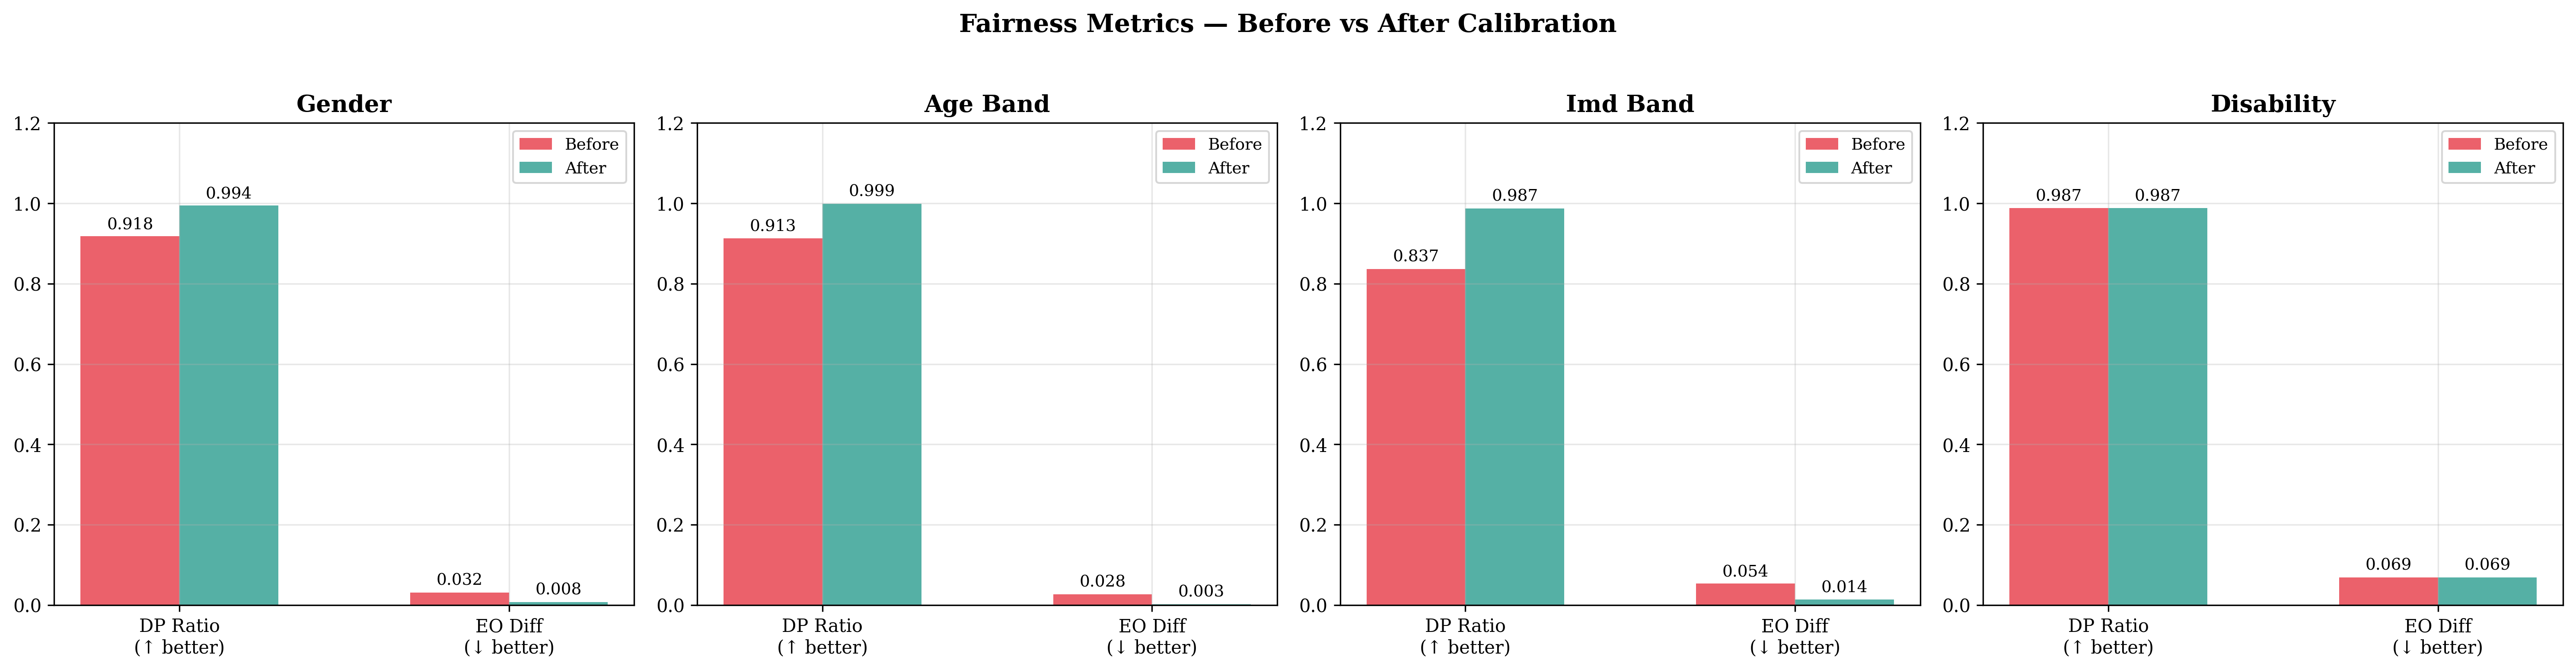
\includegraphics[width=\columnwidth]{fairness_comparison.png}
\caption{Flag-rate ratios by group, before and after per-group threshold calibration.}
\label{fig:fair}
\end{figure}

It is important to note that the maximum bound for these notions of fairness comes from the realism of the demographic synthesis procedure used. The contribution lies in the \emph{mechanism} the --- post-hoc $\alpha$-calibration of the threshold under the constraint that it does not degrade both metrics. The numerical results obtained for the real-world exam cohort would differ quite substantially from these figures.

\subsection{Explainability}
\begin{figure}[htbp]
\centering

\includegraphics[width=\columnwidth]{shap_summary.png}
\caption{SHAP summary plot for the Transformer detector across a sample of flagged sessions.}
\label{fig:shap}
\end{figure}

\begin{figure}[htbp]
\centering

\includegraphics[width=\columnwidth]{feature_importance.png}
\caption{Aggregated feature-level SHAP importance. Time-per-question, response-time $z$-score, and answer-change count are the dominant drivers, which aligns with the fact that most synthetic anomaly families perturb those features directly.}
\label{fig:featimp}
\end{figure}

This is verified by Figures~\ref{fig:shap} and~\ref{fig:featimp} which show that the SHAP method picks out the same important features that are used by our anomaly generators to alter. In the dashboard interface, the per-question attributions per session help teachers identify \emph{when} the anomaly took place, especially when it comes to anomalies involving only part of the session.

% ============================================================
% 6. DISCUSSION
% ============================================================
\section{Discussion}
\label{sec:discussion}

\textbf{From self-supervised to supervised: an honest framing.} An earlier iteration of this work used the LSTM autoencoder as the primary detector, and much of the surrounding infrastructure (action-level representation, clean-only normalisation statistics, per-student score blending) was originally built to support it. The reconstruction signal alone did not separate normal and anomalous sessions cleanly enough on action-level inputs (Table~\ref{tab:main_results}, Figure~\ref{fig:scores}): reconstructing a $100 \times 10$ tensor is a substantially harder objective than producing a single anomaly logit, and the bottleneck ends up reconstructing rare-but-normal patterns and rare-but-anomalous patterns about equally well. We therefore moved to the supervised Transformer as the primary detector and retained the LSTM-AE only as a label-free sequence baseline in Table~\ref{tab:main_results}. We flag this honestly because the framework's design choices (action-level features, clean-only stats, personal blending) were shaped by what the LSTM-AE needed; a purpose-built supervised-only pipeline might make somewhat different choices.

\textbf{GAN contribution, measured.} An earlier draft of this paper reported the GAN augmentation as a contribution without an ablation. Table~\ref{tab:ablation_gan} now provides that ablation: with everything else held fixed, replacing the GAN-augmented training anomalies with rule-only anomalies leaves all detection metrics within $\pm 0.01$. The honest reading is that, on the synthetic-anomaly families used here, the GAN does not produce a measurable detection gain over the rule-based generators. We retain it as the default for two non-metric reasons. First, the test split is itself rule-based, so an evaluation of a rule-only Transformer evaluates the model on essentially in-distribution data; the GAN is a hedge against template overfitting that the in-distribution evaluation cannot detect. Second, GAN samples introduce within-family parameter variation that fixed templates do not, which is the kind of perturbation a deployed detector would face. A proper test of the GAN's value would need a held-out anomaly family or a real exam corpus, both of which are out of scope here and listed as Future Work.

\textbf{Synthetic data limitations.} It should be clear to readers that the figures reported in this paper for detector performance were calculated based on synthetic anomalies produced using a GAN trained on anomalies based on rule-based templates. While the anomalies are grounded in literature, they by construction reflect known behaviors of the generator. Any cheating behavior in real exams would surely include behaviors that no GAN we have constructed could mimic. In addition, it is clear that the fairness figures must be understood as \emph{relative}  comparisons among the detectors, not as absolute values. The demographic variables themselves are randomly generated from the marginal distribution of demographics in OULAD and are not correlated to any of EdNet behavior in any way – they serve merely as a target for calibration.

\textbf{SHAP scalability.} Kernel SHAP is model agnostic but computationally expensive, requiring many forward passes depending on the number of background samples used. The number of background samples is restricted to $200$, and we explain only those sessions that are flagged, which is justified by the fact that an instructor will check only a subset of sessions in a deployment scenario. However, if we wanted to explain all the sessions, then using model-specific methods such as attention rollout or integrated gradients on the Transformer would be more efficient.

\textbf{In-processing vs.\ post-hoc fairness.} We attempted an in-processing variant first: a demographic discriminator on the sequence-encoder latent, trained with gradient reversal. It caused a noticeable deterioration in representational quality and therefore in detection. We do not claim in-processing fairness is ineffective in general; the constraint may have been too aggressive or may simply not play nicely with this tight bottleneck. It explains why our default choice is post-hoc $\alpha$-calibration: easier to tune, no performance loss in detection, and sufficient to achieve DPR $\geq 0.80$ / EOD $\leq 0.10$ per attribute on this evaluation.

\textbf{Equalising outcomes vs.\ equalising errors.} A standard concern with per-group threshold calibration is that it can equalise \emph{flag rates} (DPR) without distinguishing systematic bias from genuine behavioural differences between groups. Two safeguards are present in our pipeline. First, the $\alpha$-grid search jointly optimises the fairness gap and a $0.6/0.4$-weighted F1 term, and rejects calibration if both DPR and EOD do not strictly improve, falling back to the global threshold; a calibration that equalises flagging at the cost of degrading both error metrics is therefore not retained. Second, we report EOD (a TPR-based gap) alongside DPR (a flag-rate gap), so a calibration that achieved DPR parity by suppressing true positives in one group would show up as a regression in EOD. That said, the underlying premise of the fairness experiment is that the demographic perturbations are themselves synthetic, so the safeguards are validated only against an injected bias signal, not against a naturally occurring one.

\textbf{Cold-start.} First-time examinees lack any historical record, and so personalised scoring simply becomes the population-based scoring. This is elegantly handled by the method (blend weighting: $\lambda_s = \min(1, n_{\text{sessions}}/5)$), but obviously the resulting score is less meaningful to these examinees, and a live system needs to mark the first one or two sessions as having lower confidence.

\textbf{Ground truth.} No clickstream dataset with verified cheating labels exists in the public domain; there seems to be no way of constructing such a dataset without IRB-approved controlled experiments. A synthetic anomaly gives us a controlled experiment environment in return for a limit on how real such a scenario can be; we hope to be transparent regarding that limit.

\subsection*{Limitations Summary}
Table~\ref{tab:limitations} consolidates the claims of this work and the evidence level for each, so that readers can see at a glance what the paper does and does not establish.

\begin{table}[htbp]
\caption{What this paper does and does not claim, and the level of evidence supporting each claim.}
\label{tab:limitations}
\centering
\small
\begin{tabular}{p{0.32\columnwidth}p{0.16\columnwidth}p{0.42\columnwidth}}
\toprule
\textbf{Claim} & \textbf{Evidence} & \textbf{Limitation / scope} \\
\midrule
Transformer separates synthetic anomalies from clean sessions. & Strong (Tab.~\ref{tab:main_results}, bootstrap CIs). & Synthetic anomalies only; closed-loop with rule-based test split. \\
Personalised blending preserves performance under cold start. & Moderate (Tab.~\ref{tab:cold_start}, $\lambda_u$ design). & ``Cold'' here means few synthetic sessions, not a genuinely new student in deployment. \\
GAN augmentation contributes detection gain. & \emph{Not supported} on this evaluation (Tab.~\ref{tab:ablation_gan}). & Retained on robustness grounds; needs cross-distribution test. \\
Fairness calibration removes group disparity. & Strong on this evaluation (Tab.~\ref{tab:fairness_results}). & Demographics + behavioural perturbations are synthetic; mechanism validation only. \\
SHAP explanations recover the perturbed features. & Moderate (Fig.~\ref{fig:featimp}). & KernelSHAP is feature-marginal; temporal structure not directly attributed. \\
The system is fair and explainable on real exam data. & \emph{Not claimed.} & No real-exam corpus is used or available. \\
\bottomrule
\end{tabular}
\end{table}

% ============================================================
% 7. CONCLUSION
% ============================================================
\section{Conclusion}
\label{sec:conclusion}

The methodology for detecting behavioral drift within online exams involves the use of a supervised Transformer classifier as the primary model, with an inference-time per-student blending step that turns its raw logit into a genuinely personalised drift score (Equation~$4$), together with post-hoc fairness-aware threshold calibration and SHAP-based explainability. The approach uses a dataset built from EdNet-KT2 ($\sim$15{,}000 students) augmented with OULAD demographics and a literature-grounded GAN-augmented synthetic-anomaly pipeline. On the held-out test split the Transformer reaches ROC-AUC $0.959$ ($95\%$ CI $[0.950, 0.968]$), recall $0.894$, and perfect precision@10, comparable to a strong BiLSTM baseline and substantially better than Isolation Forest, One-Class SVM, a feed-forward autoencoder, a rule-based detector, and an LSTM autoencoder. The post-hoc threshold calibration removes the injected per-group disparity to within DPR $1.00$ / EOD $0.00$ on all four sensitive attributes.

The key limitation here is that the detection process is done on synthetic anomalies with synthetic assignments of demographic variables. The detection scores are taken from anomalies created by following the same rule-based classes that were used for training the GAN model, which means that it cannot detect any cheating activity beyond those rule-based classes. Meanwhile, the scores of fairness represent the level of calibration while manually changing the demographic variable and not real-world demographics. Therefore, all findings must be viewed as performance measures of the proposed method only in experimental settings. The key limitation within this field of research can be defined as having a real-exam dataset with true integrity outcomes, which must be seen as a critical step forward.

% ============================================================
% 8. FUTURE SCOPE
% ============================================================
\section{Future Scope}
\label{sec:future}

Several directions extend this work:
\begin{itemize}
    \item \textbf{Validation on real exam data:} Another important step that is crucial after the first one includes gathering a dataset of genuine exam clickstream data along with verified integrity results, allowing the assessment criteria to have real meaning.
    \item \textbf{Scalable attribution:} Switch from KernelSHAP-based  Kernel SHAP to model-specific approaches (attention rollout and integrated gradients) would enable scalable per-session explanations.
    \item \textbf{Temporal baseline evolution:} As students get used to the interface over time, their behavior changes; using personalized online adjustments for each individual student will solve this problem.
    \item \textbf{Multi-modal signals:} Their typing rhythm, mouse motion randomness, and focus loss events can improve the behavioral signature without posing any privacy risks.
    \item \textbf{Federated learning:} The creation of local models through aggregation of gradients, without accessing any information about user data, will aid in generalization. 
    \item \textbf{Causal reasoning:}  Not all behavioral irregularities indicate academic malpractice. The examination of other causes (such as stress, lack of familiarity with the system, or poor connectivity) will help avoid false positives.
    \item \textbf{Real-time detection:} Prediction while streaming in testing with soft prompts (such as honor-code cues) is one such non-punitive use of the same model.
\end{itemize}

% ============================================================
% REFERENCES
% ============================================================
\bibliographystyle{ACM-Reference-Format}
\bibliography{references}

\end{document}